% SIAM UQ Manuscript using the official SIAM class siamart251216.cls
\documentclass[review,hidelinks,onefignum,onetabnum]{siamart251216}

% Packages
\usepackage{amsmath,amssymb}
\usepackage{mathtools}
\usepackage{bm}
\usepackage{graphicx}
\usepackage{booktabs}
\usepackage{enumitem}
\usepackage{algorithm}
\usepackage{algpseudocode}
\usepackage{xr-hyper}
\usepackage{xcolor}
\externaldocument[S-]{part1_supplement}

% Math macros
\newcommand{\RR}{\mathbb{R}}
\newcommand{\NN}{\mathbb{N}}
\newcommand{\EE}{\mathbb{E}}
\newcommand{\PP}{\mathbb{P}}
\newcommand{\Var}{\mathrm{Var}}
\newcommand{\Cov}{\mathrm{Cov}}
\newcommand{\DKL}{\mathcal{D}_{\mathrm{KL}}}
\newcommand{\tr}{\operatorname{Tr}}
\newcommand{\diag}{\mathrm{diag}}
\newcommand{\divop}{\operatorname{div}}
\DeclareMathOperator*{\argmin}{arg\,min}
\DeclareMathOperator*{\argmax}{arg\,max}
\newcommand{\gauss}{\gamma}
\renewcommand{\vec}[1]{\bm{#1}}

% SIAM convention: finite-dimensional matrices and vectors in bold.
% Used selectively for central discrete linear-algebraic objects
% (e.g. Hyvärinen system A\theta=b, the copula-score covariance C,
% the BIP forward matrix A). Not all vectors/matrices use these —
% densities, operator-valued things, and scalar-valued functions
% remain non-bold by convention.
% --- Matrices
\newcommand{\mA}{\bm{A}}
\newcommand{\mb}{\bm{b}}
\newcommand{\mh}{\bm{h}}
\newcommand{\mC}{\bm{C}}
\newcommand{\mB}{\bm{B}}
\newcommand{\hmC}{\widehat{\bm{C}}}
\newcommand{\mV}{\bm{V}}
\newcommand{\hmV}{\widehat{\bm{V}}}
\newcommand{\whmV}{\widehat{\bm{V}}}
\newcommand{\mL}{\bm{L}}
\newcommand{\mP}{\bm{P}}
\newcommand{\hmP}{\widehat{\bm{P}}}
\newcommand{\mS}{\bm{S}}
\newcommand{\mU}{\bm{U}}
\newcommand{\mQ}{\bm{Q}}
\newcommand{\cond}{\operatorname{cond}}
\newcommand{\mI}{\bm{I}}
\newcommand{\mW}{\bm{W}}
\newcommand{\mR}{\bm{R}}
\newcommand{\mD}{\bm{D}}
\newcommand{\mG}{\bm{G}}
\newcommand{\mH}{\bm{H}}
\newcommand{\mPhi}{\bm{\Phi}}
\newcommand{\mPsi}{\bm{\Psi}}
\newcommand{\mLambda}{\bm{\Lambda}}
\newcommand{\mM}{\bm{M}}
\newcommand{\hbeta}{\widehat{\beta}}
\DeclareMathOperator{\range}{range}
% --- Manifolds of frames / subspaces
\newcommand{\St}{\mathrm{St}}
\newcommand{\Gr}{\mathrm{Gr}}
% --- Vectors
\newcommand{\vtheta}{\bm{\theta}^{d}}
\newcommand{\hvtheta}{\widehat{\bm{\theta}}^{d}}
\newcommand{\whvtheta}{\widehat{\bm{\theta}}^{d}}
\newcommand{\vbeta}{\bm{\theta}^{r}}
\newcommand{\hvbeta}{\widehat{\bm{\theta}}^{r}}
\newcommand{\whvbeta}{\widehat{\bm{\theta}}^{r}}
% --- Noise / observation / rank-Gaussianized vectors (bold)
\newcommand{\vn}{\bm{n}}
\newcommand{\vN}{\bm{N}}
\newcommand{\vx}{\bm{x}}
\newcommand{\vX}{\bm{X}}
\newcommand{\vy}{\bm{y}}
\newcommand{\vY}{\bm{Y}}
\newcommand{\vz}{\bm{z}}
\newcommand{\vZ}{\bm{Z}}
\newcommand{\vu}{\bm{u}}
\newcommand{\vU}{\bm{U}}
\newcommand{\vv}{\bm{v}}
\newcommand{\vw}{\bm{w}}
\newcommand{\vW}{\bm{W}}
\newcommand{\vF}{\bm{F}}
% --- Score / log-copula operators (mathcal, not bold)
\newcommand{\scZ}{\mathcal{Z}}
\newcommand{\scL}{\mathcal{L}}
\newcommand{\scS}{\mathcal{S}}
\newcommand{\scF}{\mathcal{F}}

\setlength{\emergencystretch}{3em}

% Oxford comma via cleveref (SIAM template convention)
\newcommand{\creflastconjunction}{, and~}

% SIAM-predefined environments: theorem, proposition, lemma, corollary, definition (already in class file).
% Declare our additional environments using the SIAM macros.
\newsiamremark{remark}{Remark}
\newsiamremark{assumption}{Assumption}
\crefname{remark}{Remark}{Remarks}
\crefname{assumption}{Assumption}{Assumptions}
% Cleveref types labels in \newsiamremark environments by the shared theorem
% counter, so \Cref of a remark or assumption prints "Theorem N". Alias the
% counter to the correct type inside each environment (the alias is local to
% the environment group), which makes \Cref print Remark/Assumption.
\let\origremarkenv\remark
\renewcommand{\remark}{\crefalias{theorem}{remark}\origremarkenv}
\let\origassumptionenv\assumption
\renewcommand{\assumption}{\crefalias{theorem}{assumption}\origassumptionenv}
\crefname{appendix}{Appendix}{Appendices}
\Crefname{appendix}{Appendix}{Appendices}

% Running headers (short title, short author list)
\headers{Copula Active Subspaces}{J.~Chen and P.~J.~van Leeuwen}

% Title and authors
\title{Copula Active Subspaces I: A Score-Covariance Method for Reduced-Order Non-Gaussian Density Estimation\thanks{Submitted to the editors \today. This is Part~I of a two-part work; the companion paper \emph{Copula Active Subspaces II: Error Decomposition, A Posteriori Estimation, and Sharpness of the Bounds} develops the finite-sample analysis. \funding{This work was supported by the Consortium for Advanced Data Assimilation Research and Education (CADRE), funded by NOAA under grant 2007893.}}}

\author{%
  Joshua Chen\thanks{Department of Atmospheric Science, Colorado State University, Fort Collins, CO 80523 (\email{Joshua.Chen@colostate.edu}).}
  \and
  Peter Jan van Leeuwen\thanks{Department of Atmospheric Science, Colorado State University, Fort Collins, CO 80523 (\email{Peter.vanLeeuwen@colostate.edu}).}
}

\begin{document}
\maketitle

\begin{abstract}
In Bayesian inference problems with non-Gaussian observation noise, the posterior is only as accurate as the noise density, and gradient-based samplers need that density and its gradient evaluable pointwise, whether from an explicit expression or from code, and without an inner solve. We propose Copula Active Subspaces (\textsc{Cas}) to represent this noise density. A componentwise rank transform isolates the noise law's dependence in its copula, and a rank-$r$ reduction keeps only the directions along which that dependence varies. These directions are the leading eigenvectors of the copula score covariance $\mC := \Cov_{\pi_{\vZ}}(\nabla\log c^{Z})$, which is what makes the reduction a copula active subspace. Because $\mC$ vanishes when the coordinates are independent, these are directions of dependence, which the covariance of the data need not identify. Applied to the copula, the Gaussian-reference KL divergence bound of certified dimension reduction holds with the explicit constant $\tfrac12$ and is minimized over all rank-$r$ reductions by exactly this eigenspace. We give a diagnostic of the remaining truncation error that is computable from the samples alone. Hermite score matching then yields the reduced log-density and its gradient in closed form, with the truncation orders and the Stage-2 regularization constants chosen on validation samples. The reduction replaces a $d$-dimensional density estimation problem by an $r$-dimensional one. On a $d=20$ noise law and a Bayesian inference problem with that noise, \textsc{Cas} lowers noise KL divergence more than fivefold and posterior KL divergence more than sevenfold against Gaussian-copula, product-of-marginals, and PCA-subspace baselines, and lowers noise KL divergence by factors of about $3.5$ and $2.7$ on two further $d=20$ examples.
\end{abstract}

\begin{keywords}
copula, active subspace, score matching, dimension reduction, Hermite polynomials, Bayesian inference problems, non-Gaussian observation error
\end{keywords}

\begin{MSCcodes}
62G07, 62H05, 62H12, 62B10, 60E15, 62F15
\end{MSCcodes}

% =====================================================================
\section{Introduction}
\label{sec:intro}

In a Bayesian inference problem, a prior on an unknown inference variable $\vx$ is updated by the information that an observation $\vy = \mathcal{G}(\vx) + \vn$ provides about it, where the noise $\vn \in \RR^d$ has law $\pi_{\vn}$. Non-Gaussian noise is common in remote sensing \cite{BormannBauerGeer2011}, data assimilation \cite{JanjicBormannBocquet2018survey, HuVanLeeuwenGeer2024, FowlerVanLeeuwen2013}, and image reconstruction \cite{KaipioSomersaloBook}. A Gaussian likelihood then misstates the noise law, and no choice of its covariance repairs the misstatement, since the Gaussian family does not contain $\pi_{\vn}$. If $\pi_{\vn}$ in the likelihood is replaced with a candidate $\widehat\pi_{\vn}$ and $\widehat\pi_{X|Y}$ denotes the resulting posterior, the KL divergence chain rule gives
\begin{equation}
  \EE_{\vy\sim \pi_Y}\!\left[\DKL\!\left(\pi_{X|Y}(\cdot\mid\vy) \,\big\|\, \widehat\pi_{X|Y}(\cdot\mid\vy)\right)\right]
  \;\le\; \DKL(\pi_{\vn}\,\|\,\widehat\pi_{\vn}),
  \label{eq:posterior-noise-kl}
\end{equation}
so the average posterior divergence is bounded by that of the noise estimate.\footnote{Apply the KL divergence chain rule to the joint laws $\pi(\vx,\vy) = \pi_X(\vx)\,\pi_{\vn}(\vy - \mathcal G(\vx))$ and $\widehat\pi(\vx,\vy) = \pi_X(\vx)\,\widehat\pi_{\vn}(\vy - \mathcal G(\vx))$ in both orders. In the order $(\vx,\vy)$ it gives $\DKL(\pi\,\|\,\widehat\pi) = \DKL(\pi_{\vn}\,\|\,\widehat\pi_{\vn})$, by translation invariance of the KL divergence; in the order $(\vy,\vx)$ it gives the left side of \eqref{eq:posterior-noise-kl} plus the nonnegative term $\DKL(\pi_Y\,\|\,\widehat\pi_Y)$, which the inequality of \eqref{eq:posterior-noise-kl} absorbs. Both noise laws are probability densities and $\widehat\pi_{\vn}$ is positive and bounded, so that $\widehat\pi_Y$ and the conditionals $\widehat\pi_{X|Y}$ are well defined; the estimator of \Cref{sec:estimator} is all three.} Gradient-based posterior samplers \cite{RobertsTweedie1996, Neal2011HMC, CotterRobertsStuartWhite2013} require the unnormalized log-density $\log\pi_{\vn}$ and its gradient $\nabla\log\pi_{\vn}$ in closed form, and we seek a tractable estimator of both from $N$ i.i.d.\ samples of the noise in $\RR^d$. Where the noise cannot be observed directly, those samples are approximate samples based on residuals $\vn^{(i)} = \vy^{(i)} - \mathcal G(\vx^\star)$ formed at a nominal variable value $\vx^\star$, such as a maximum-likelihood estimate or an analysis state. We take the sample as given throughout, and return in \Cref{sec:limitations} to what its construction requires. The paper accordingly concentrates on estimating $\pi_{\vn}$ itself, with \Cref{sec:exp-bip} confirming the transfer from noise divergence to posterior divergence.

In practice the noise model is commonly simplified. Univariate noise modeling treats the coordinates as independent, a Gaussian likelihood keeps only second moments, and a Gaussian copula admits arbitrary marginals but represents dependence only through a correlation matrix. Each simplification omits dependence structure, which enlarges the noise divergence on the right of \eqref{eq:posterior-noise-kl}. We reduce that divergence as follows. The $d$ univariate marginals of $\pi_{\vn}$ are classical one-dimensional estimation problems (\Cref{sec:estimator}), and the dependence among the coordinates is the $d$-dimensional problem. A componentwise rank transform separates the two. It maps the samples to coordinates $\vZ$ with standard-Gaussian marginals, so that everything left to estimate is the dependence, described by the copula density $c^{Z} := \pi_{\vZ}/\gauss_d$, where $\gauss_k$ denotes the standard Gaussian density on $\RR^k$. A rank-$r$ dimension reduction then confines that dependence to a subspace. When $c^{Z}$ varies only along $r \ll d$ directions, which is the regime considered here, those directions span an \emph{active subspace} of the copula, and the reduction leaves an $r$-dimensional estimation problem. The rest of the paper answers two questions: how to identify these directions from samples, and how to quantify the error of the reduction when the concentration is imperfect.

\paragraph{Related work} The rank transform is the standard tool of the semiparametric copula literature \cite{Sklar1959, Nelsen2006book, LiuLaffertyWasserman2009nonparanormal}, which treats marginals and dependence separately. The reduction adapts the active-subspace principle \cite{ConstantineDowWang2014, Constantine2015book, ZahmConstantinePrieurMarzouk2020, BigoniMarzoukPrieurZahm2022}, extraction of low-dimensional structure from a gradient covariance, from functions and log-densities to the copula score. Unlike likelihood-informed subspaces \cite{CuiMartinMarzoukSolonenSpantini2014, ZahmCuiLawSpantiniMarzouk2022, CuiTongZahm2022}, which locate posterior-relevant directions from forward-map gradients, the reduction here uses only residual samples. Score ratio matching \cite{BaptistaBrennanMarzouk2025} learns the score ratio $\nabla\log(\pi/\rho)$ of a density $\pi$ to a reference $\rho$ with a neural network and reduces dimension along the leading eigenvectors of the second moment of the learned ratio. For a standard Gaussian $\rho$ this second moment is the diagnostic matrix of certified dimension reduction \cite{ZahmCuiLawSpantiniMarzouk2022}. Stage~1 of \textsc{Cas} is an instance of score ratio matching. With $\pi = \pi_{\vZ}$ and $\rho = \gauss_d$, the score ratio is the copula score, its second moment is the copula score covariance $\mC$ of \Cref{sec:method}, and the Hermite score-matching objective \eqref{eq:hyv-quadratic} equals, up to an additive constant, the score-ratio-matching objective of \cite[Thm.~3.2]{BaptistaBrennanMarzouk2025}. \textsc{Cas} adds two elements to this setting. The componentwise rank transform comes first, after which $\gauss_d$ matches every marginal and $\mC$ vanishes under independence. The model is a Hermite polynomial class with a Tikhonov penalty, on which the objective is quadratic and is minimized in closed form without training a network. Among non-Gaussian density-reduction methods, transport-based inference and lazy maps \cite{MarzoukMoselhyParnoSpantini2016, MorrisonBaptistaMarzouk2017, BaptistaMarzoukZahm2023representation, BrennanBigoniZahmSpantiniMarzouk2020} are the closest relatives. Ours is a Hermite polynomial counterpart, estimated by regularized linear solves, with a closed-form likelihood.

\paragraph{Contributions}
\begin{enumerate}[leftmargin=*,topsep=2pt,itemsep=2pt]
\item \emph{A two-stage estimator of the copula.} A componentwise rank transform isolates the noise law's dependence in its copula density, which we reduce to a low-dimensional subspace and estimate by Hermite copula score matching, returning the reduced log-density and its gradient in closed form for gradient-based posterior samplers.

\item \emph{Bound-optimal dimension reduction with a closed-form diagnostic.} Applied to the copula, the Gaussian-reference KL divergence bound of certified dimension reduction \cite{ZahmCuiLawSpantiniMarzouk2022} has the explicit constant $\tfrac12$, and its minimizer over rank-$r$ subspaces is the leading eigenspace of the copula score covariance. We give a closed-form, sample-computable diagnostic of the rank-$r$ truncation error.

\item \emph{Empirical validation.} \textsc{Cas} improves noise KL divergence more than fivefold and posterior KL divergence more than sevenfold over Gaussian-copula, product-of-marginals, and PCA-subspace baselines, on a $d=20$ non-Gaussian copula example problem and a Bayesian inference problem with the same noise, and the gains persist across three structurally distinct noise laws.
\end{enumerate}

\Cref{sec:method} constructs the reduction and its bound-optimal subspace, \Cref{sec:estimator} builds the two-stage estimator, and \Cref{sec:theory} identifies the rank-$r$ truncation error of the reduction and the closed-form diagnostic that estimates it. \Cref{sec:experiments} measures subspace recovery, noise divergence, and posterior accuracy on three example problems.

% =====================================================================
\section{Copula dimension reduction}
\label{sec:method}

This section concerns the true law $\pi_{\vn}$, before any estimation enters. One matrix is central, the copula-score covariance $\mC$: it equals zero exactly when the coordinates are independent, and its top-$r$ eigenspace minimizes a KL divergence bound over all rank-$r$ reductions (\Cref{thm:kl-trunc}, \Cref{cor:optimal-subspace}).

Given continuous univariate marginal CDFs $F_1,\ldots,F_d: \RR\to(0,1)$ and i.i.d.\ samples $\{\vn^{(k)}\}_{k=1}^N \subset \RR^d$ from $\pi_{\vn}$, the componentwise rank transform
\begin{equation}
  \scZ: \RR^d \to \RR^d, \qquad
  \scZ(\vx)_i := \Phi^{-1}\bigl(F_i(x_i)\bigr), \quad i=1,\ldots,d,
  \label{eq:rank-transform}
\end{equation}
sends $\pi_{\vn}$ to a measure $\pi_{\vZ}$ with standard-Gaussian marginals and the same copula \cite{Sklar1959, Nelsen2006book}, separating marginal estimation from dependence estimation, and we say the transform \emph{rank-Gaussianizes} the marginals. The ranks of the sample, and therefore the rank-transformed sample, are unchanged under coordinatewise strictly increasing transformations of the residuals \cite{LiuLaffertyWasserman2009nonparanormal}. Two properties of the $\vZ$-coordinates are used throughout: $\gauss_d$ factorizes as $\gauss_r\otimes\gauss_{d-r}$ under any splitting of $\RR^d$ into an $r$-dimensional subspace and its orthogonal complement, which the rank-$r$ reduction relies on, and the Hermite polynomial basis of \Cref{sec:method-core} is orthonormal in $L^2(\gauss_d)$.

In $\vZ$-coordinates, writing $c^{Z} := \pi_{\vZ}/\gauss_d$ for the copula density on standard-Gaussian marginals,\footnote{Sklar's theorem writes $\pi_{\vZ}(\vz) = c(\Phi(z_1),\dots,\Phi(z_d))\,\gauss_d(\vz)$ with $c$ a density on $[0,1]^d$, on the uniform arguments $\Phi(z_i)$. We work in the rank-Gaussianized coordinates and write $c^{Z}(\vz) := \pi_{\vZ}(\vz)/\gauss_d(\vz) = c(\Phi(\vz))$, calling $c^{Z}$ the copula, $\scL = \log c^{Z}$ the log-copula, and $\scS = \nabla_{\vz}\scL = \nabla\log\pi_{\vZ} + \vz$ the copula score. The reduced analogue $c^{U}_r(\vu) := \pi_{\vU}(\vu)/\gauss_r(\vu)$ on $\vu = \mV_r^\top\vz$ is likewise a density relative to $\gauss_r$, not a copula density in the strict uniform-margin sense.} we define the log-copula $\scL: \RR^d\to\RR$, the copula score $\scS: \RR^d\to\RR^d$, and the symmetric positive semidefinite copula-score covariance $\mC\in\RR^{d\times d}$:
\begin{equation}
\begin{gathered}
  \scL(\vz) := \log c^{Z}(\vz),\qquad
  \scS(\vz) := \nabla \scL(\vz),\\[2pt]
  \mC := \Cov_{\pi_{\vZ}}\!\bigl(\scS(\vZ)\bigr) \;=\; \EE_{\pi_{\vZ}}\bigl[\scS(\vZ)\otimes\scS(\vZ)\bigr],
\end{gathered}
  \label{eq:L-T-C-def}
\end{equation}
under the regularity assumption below; the two forms in \eqref{eq:L-T-C-def} coincide because the copula score is centered ($\EE_{\pi_{\vZ}}[\scS] = 0$, as $\nabla\log\pi_{\vZ}$ integrates to zero, \Cref{app:regularity}, and $\pi_{\vZ}$ has zero-mean marginals). The score vanishes a.e.\ under independence ($\scL\equiv 0$), and conversely $\mC = 0$ forces $\scS = 0$ a.e., so $\mC$ is zero exactly under independence. For a unit direction $\vv\in\RR^d$, $\vv^\top\mC\vv = \EE_{\pi_{\vZ}}[(\partial_{\vv}\scL)^2]$ is the mean squared derivative of the log-copula along $\vv$, equal to zero if and only if $\partial_{\vv}\scL = 0$ a.e., that is, if and only if $c^{Z}$ does not vary along $\vv$. $\mC$ is an average gradient outer product, and the same object appears in the diagnostic matrices of gradient- and likelihood-informed dimension reduction \cite{ZahmConstantinePrieurMarzouk2020, BigoniMarzoukPrieurZahm2022, ChenArnaudBaptistaZahm2024} (which use forward-map and log-likelihood gradients) and in the feature-learning mechanism of \cite{RadhakrishnanBeagleholePanditBelkin2024}.

We use the following regularity conditions on the log-copula.

\begin{assumption}[Regularity of the log-copula]
\label{ass:tempered}
The copula density $c$ of $\pi_{\vn}$ is strictly positive on $(0,1)^d$, the log-copula $\scL = \log(c\circ\Phi)$ is continuously differentiable on $\RR^d$, and:
\textup{(T1)} \emph{pointwise sub-Gaussian density bound}, $\pi_{\vZ}(\vz) \le K_0(1+\|\vz\|^{2m})\gauss_d(\vz/\sigma_0)$ for some $K_0\ge 1$, $\sigma_0>1$, $m\ge 0$; \textup{(T2)} \emph{polynomial growth of the score}, $\|\nabla\scL(\vz)\|_2 \le \alpha' + \beta'\|\vz\|^q$ for some $\alpha', \beta' \ge 0$, $q\in\NN$.
\end{assumption}

\noindent (T1)--(T2) give $\scL\in L^2(\gauss_d)$ and $\scS \in L^2(\pi_{\vZ};\RR^d)$, and in particular $\tr(\mC)<\infty$ (\Cref{app:regularity}), as needed for \eqref{eq:L-T-C-def} to be finite. The density bound (T1) excludes heavier-than-Gaussian tails. The technical consequences that follow from this assumption are collected in \Cref{app:regularity}.

$\mC$ is defined and finite under Assumption~\ref{ass:tempered}; we now state the dimension reduction it motivates. A rank-$r$ dimension reduction approximates $\pi_{\vn}$ within the family whose copula factor depends on only $r$ projected coordinates. It is specified by a matrix $\mV_r$ with $r$ orthonormal columns, $\mV_r^\top\mV_r = \mI_r$, together with a density on the \emph{active subspace} $\mathrm{span}(\mV_r)$; we write $\St(r,\RR^d)$ for the set of such matrices and $\Gr(r,\RR^d)$ for the set of rank-$r$ subspaces of $\RR^d$. The rank $r$ trades approximation accuracy against the statistical error of estimating the reduced density from $N$ samples: at $r=0$ the family is the product of marginals $\prod_i\pi_i$ and carries no dependence, the univariate noise estimation common in practice; at $r=d$ it contains the exact joint law and a full $d$-dimensional density must be estimated; intermediate $r$ retains the $r$ leading dependence directions. The bound-optimal reduced density has two ingredients: the best density on a given $\mV_r$ (\Cref{sec:reduced-form}), and the subspace itself, the minimizer of a KL divergence upper bound, which is the top-$r$ eigenspace of $\mC$ (\Cref{sec:kl-trunc}).

\subsection{Reduced model form}
\label{sec:reduced-form}

The \emph{reduced-model space} for a given $\mV_r \in \St(r,\RR^d)$, rank transform $\scZ$, and marginals $\{\pi_i\}$ is
\begin{equation}
  \mathcal M(\mV_r, \scZ, \{\pi_i\}) \;:=\; \Bigl\{\, \pi : \pi(\vx) = c'\bigl(\mV_r^\top \scZ(\vx)\bigr)\textstyle\prod_{i=1}^d \pi_i(x_i)\,\Bigr\},
  \label{eq:reduced-form}
\end{equation}
where $c'$ ranges over probability densities on $\RR^r$ with respect to $\gauss_r$. Here and throughout, $c$ with a superscript denotes a copula-type density relative to the Gaussian reference of matching dimension, the prime marks a generic member of the family \eqref{eq:reduced-form}, and hats mark estimates; the optimal member $c_r^{U}$ is identified below. Set the \emph{active coordinates} $\vU := \mV_r^\top\vZ$ and the \emph{complement coordinates} $\vW := \mV_\perp^\top\vZ$, where $\mV_\perp \in \St(d-r,\RR^d)$ is an orthonormal completion of $\mV_r$, $[\mV_r\ \mV_\perp] \in \mathrm{O}(d)$. Under the Gaussian reference the two blocks are independent, $\gauss_d = \gauss_r\otimes\gauss_{d-r}$ with $\vU\sim\gauss_r$ and $\vW\sim\gauss_{d-r}$; write $\pi_{\vW\mid\vU}$ for the conditional law of $\vW$ given $\vU$ under $\pi_{\vZ}$. In these coordinates a member of $\mathcal M(\mV_r, \scZ, \{\pi_i\})$ has $\vZ$-density $c'(\vu)\,\gauss_d(\vz)$: it places an arbitrary marginal $c'\gauss_r$ on the active coordinates and fixes $\vW\mid\vU \sim \gauss_{d-r}$, independent of $\vU$, on the complement. Splitting the KL divergence from $\pi_{\vZ}$ into the divergence of the $\vU$-marginals plus the $\vU$-averaged divergence of the conditionals (the chain rule), the marginal term equals zero at the choice $c' = c_r^{U} := \pi_{\vU}/\gauss_r$, and the conditional term is the same for every member of the family. The KL divergence projection of $\pi_{\vn}$ onto $\mathcal M(\mV_r, \scZ, \{\pi_i\})$ is therefore
\begin{equation}
  \pi_{\vn}(\vx;\mV_r) := c_r^{U}\!\bigl(\mV_r^\top \scZ(\vx)\bigr) \prod_{i=1}^d \pi_i(x_i),
  \label{eq:pi-star-form}
\end{equation}
with residual exactly the conditional term $\EE_{\pi_{\vU}}[\DKL(\pi_{\vW\mid\vU}\,\|\,\gauss_{d-r})]$, so the reduction is exact precisely when $c^{Z}$ does not vary along the complement. The optimality here is over the reduced factor $c'$ within $\mathcal M(\mV_r, \scZ, \{\pi_i\})$, not over the family itself. Every member of the family fixes $\vW\mid\vU\sim\gauss_{d-r}$, so the conditional term is common to all of them and no choice of $c'$ affects it, and $c' = c_r^{U}$ is the member that sets the remaining term to zero. Which subspace to retain the dependence on is the separate question, answered in \Cref{sec:kl-trunc}.

\subsection{KL divergence upper bound and optimal subspace}
\label{sec:kl-trunc}

\begin{theorem}[KL divergence upper bound on the reduced model]
\label{thm:kl-trunc}
Under Assumption~\ref{ass:tempered}, for every $\mV_r \in \St(r,\RR^d)$,
\begin{equation}
  \DKL\bigl(\pi_{\vn} \,\|\, \pi_{\vn}(\,\cdot\,;\mV_r)\bigr) \;\leq\; \tfrac{1}{2}\,\tr\!\bigl((\mI - \mV_r\mV_r^\top)\,\mC\bigr).
  \label{eq:kl-trunc}
\end{equation}
\end{theorem}

\emph{Proof.} See \Cref{app:thm-trunc}. Applying the subspace KL divergence bound of \cite[Cor.~2.10]{ZahmCuiLawSpantiniMarzouk2022}, which follows from the subspace logarithmic Sobolev inequality of \cite[Thm.~2.9]{ZahmCuiLawSpantiniMarzouk2022}, to the copula density $\pi_{\vZ}$ relative to the Gaussian reference $\gauss_d$ gives \eqref{eq:kl-trunc}, with the copula-score covariance $\mC$ as the diagnostic second-moment matrix.

The reduced model \eqref{eq:pi-star-form} keeps the active marginal $\pi_{\vU}$ exact and replaces only the complement law by $\gauss_{d-r}$, so the bounded divergence is the $\vU$-average $\EE_{\pi_{\vU}}[\DKL(\pi_{\vW\mid\vU}\,\|\,\gauss_{d-r})]$. The prefactor of the general bound is a log-Sobolev constant of the reference conditionals; here that reference is the exact $\gauss_{d-r}$, whose log-Sobolev constant is the sharp value $1$ \cite[Prop.~5.5.1]{BakryGentilLedoux2014}, going back to \cite{Gross1975}, so \eqref{eq:kl-trunc} carries the explicit factor $\tfrac12$ rather than an unknown prefactor. This factor arises in \Cref{app:thm-trunc} from two places: the logarithmic Sobolev inequality contributes the factor $2$ in $\DKL \le 2\,\EE_{\gauss}[\|\nabla\sqrt{g}\|^2]$, and $h := \sqrt{\pi_{\vZ}/\gauss_d}$ has $\nabla h = \tfrac12 h\,\scS$, contributing $\tfrac14$ once squared; thus the product is $\tfrac12$.

\begin{corollary}[Bound-optimal subspace]
\label{cor:optimal-subspace}
Let $(\lambda_i(\mC), \vv_i(\mC))_{i=1}^d$ be the eigenpairs of $\mC$ ordered $\lambda_1(\mC) \ge \cdots \ge \lambda_d(\mC)$, and $\mV_r^{\mC} := [\vv_1(\mC)\,\cdots\,\vv_r(\mC)]$. The bound of \Cref{thm:kl-trunc} depends only on $\mathrm{span}(\mV_r) \in \Gr(r,\RR^d)$; its minimum is attained on $\mathrm{span}(\mV_r^{\mC})$ with value
\[
  \tfrac{1}{2}\tr\!\bigl((\mI-\mV_r^{\mC}\mV_r^{\mC\top})\mC\bigr) \;=\; \tfrac{1}{2}\sum_{i > r}\lambda_i(\mC),
\]
giving $\DKL\bigl(\pi_{\vn}\,\|\,\pi_{\vn}(\,\cdot\,;\mV_r^{\mC})\bigr) \leq \tfrac{1}{2}\sum_{i>r}\lambda_i(\mC)$.
\end{corollary}

\emph{Proof.} The bound of \Cref{thm:kl-trunc} depends on $\mV_r$ only through $\mathrm{span}(\mV_r)$, and minimizing $\tr((\mI-\mP)\mC)$ over rank-$r$ orthogonal projectors is the Eckart--Young low-rank approximation problem in the Frobenius norm \cite{EckartYoung1936}: writing $\mC = \mC^{1/2}\mC^{1/2}$, the quantity $\tr((\mI-\mP)\mC) = \|(\mI-\mP)\mC^{1/2}\|_F^2$ is the squared Frobenius distance from $\mC^{1/2}$ to its projection onto a rank-$r$ subspace, minimized by the top-$r$ eigenspace of $\mC$ with minimum $\sum_{i>r}\lambda_i(\mC)$.

We call $\mathrm{span}(\mV_r^{\mC})$ the \emph{copula active subspace}. The reduction is lossless when the tail eigenvalues $\lambda_{r+1}(\mC),\ldots,\lambda_d(\mC)$ vanish: $\pi_{\vn}(\vx) = \pi_{\vn}(\vx;\mV_r^{\mC})$ a.e. The bound \eqref{eq:kl-trunc} therefore has two uses: its minimizer is the subspace, in closed form, and its value at that minimizer bounds the divergence the reduction incurs. Both results are formulated using the exact score covariance $\mC$, and \Cref{sec:theory} develops the consequences of \Cref{thm:kl-trunc} for an estimated basis $\hmV_r^{\mC}$.

% =====================================================================
\section{The \textsc{Cas} estimator}
\label{sec:estimator}

The estimator has three parts, each depending on the one before: estimated marginals, the empirical distribution functions $\{\widehat F_i\}$ that define the empirical rank transform $\widehat\scZ$ (\Cref{alg:cas}, step~1) and the kernel density estimates $\{\widehat\pi_i\}$; a basis $\hmV_r^{\mC}$ for the estimated Stage-1 subspace, computed from the rank-Gaussianized samples by Hermite copula score matching (Stage 1, \Cref{sec:method-core}); and the reduced log-density $\scL_r := \log c_r^{U} = \log(\pi_{\vU}/\gauss_r)$ on $\RR^r$, estimated on the projected coordinates $\vU = \hmV_r^{\mC\top}\vZ$ with the regularizer of \Cref{sec:ridge} (Stage 2, \Cref{sec:reduced-model}). The full estimator is
\begin{equation}
\begin{gathered}
  \log\widehat\pi_{\vn}(\vx;\hmV_r^{\mC}) = \widehat{\scL}_r(\hmV_r^{\mC\top}\widehat\scZ(\vx)) + \sum_i\log\widehat\pi_i(x_i) - \log\widehat Z_{\vn},\\[2pt]
  \widehat Z_{\vn} := \int_{\RR^d} e^{\widehat{\scL}_r(\hmV_r^{\mC\top}\widehat\scZ(\vx))}\prod_i\widehat\pi_i(x_i)\,d\vx.
\end{gathered}
  \label{eq:cas-estimator}
\end{equation}
The normalizer $\widehat Z_{\vn}$ is a constant, so it enters the log-density but not its gradient, and it is finite because the empirical transform $\widehat\scZ$ takes values in a bounded box, on which the polynomial $\widehat\scL_r$ is bounded. The transform $\widehat\scZ$ and the kernel estimates $\widehat\pi_i$ are estimated separately, so the normalization of the family \eqref{eq:reduced-form} does not carry over to their composition, and \eqref{eq:cas-estimator} normalizes the composition directly. When $\widehat Z_r := \int_{\RR^r} e^{\widehat\scL_r}\,d\gauss_r$ is finite, normalizing the reduced factor $e^{\widehat\scL_r}/\widehat Z_r$ first gives the same density, since that constant cancels. The estimate is thus a probability density, positive, and bounded, since each kernel density estimate $\widehat\pi_i$ is bounded; these are the conditions required by \eqref{eq:posterior-noise-kl}.

\paragraph{Marginals} Estimating the $d$ marginals is the classical part of the composition, with rates available for kernel and log-spline density estimation \cite{Hall1987, Stone1990}. Each $\widehat\pi_i$ is a Gaussian-kernel density estimator with a robust Silverman bandwidth $h\asymp N^{-1/5}$ \cite[\S 3.4]{Silverman1986}, and $\widehat F_i$ is the empirical distribution function of \Cref{alg:cas}, step~1 (\Cref{app:protocol}). The KL divergence these estimates contribute is not analyzed here (\Cref{sec:limitations}).

\subsection{Stage 1: subspace identification}
\label{sec:method-core}

Stage 1 returns $\hmV_r^{\mC}$, the matrix of top-$r$ eigenvectors of the empirical score second-moment matrix $\hmC$, whose column space is the estimated Stage-1 subspace analyzed in \Cref{sec:theory}, and \Cref{fig:pedagogical} illustrates it in two dimensions. Stage 1 computes $\hmC$ in closed form from the samples in three steps: the log-copula is expanded in a Hermite polynomial basis; its coefficients are recovered by score matching as a single linear system; and $\hmC$ is assembled from the resulting analytical scores. \Cref{app:stage2-foundations} gives the score-matching identity and the explicit linear system behind the second step.

\begin{figure}[t]
\centering
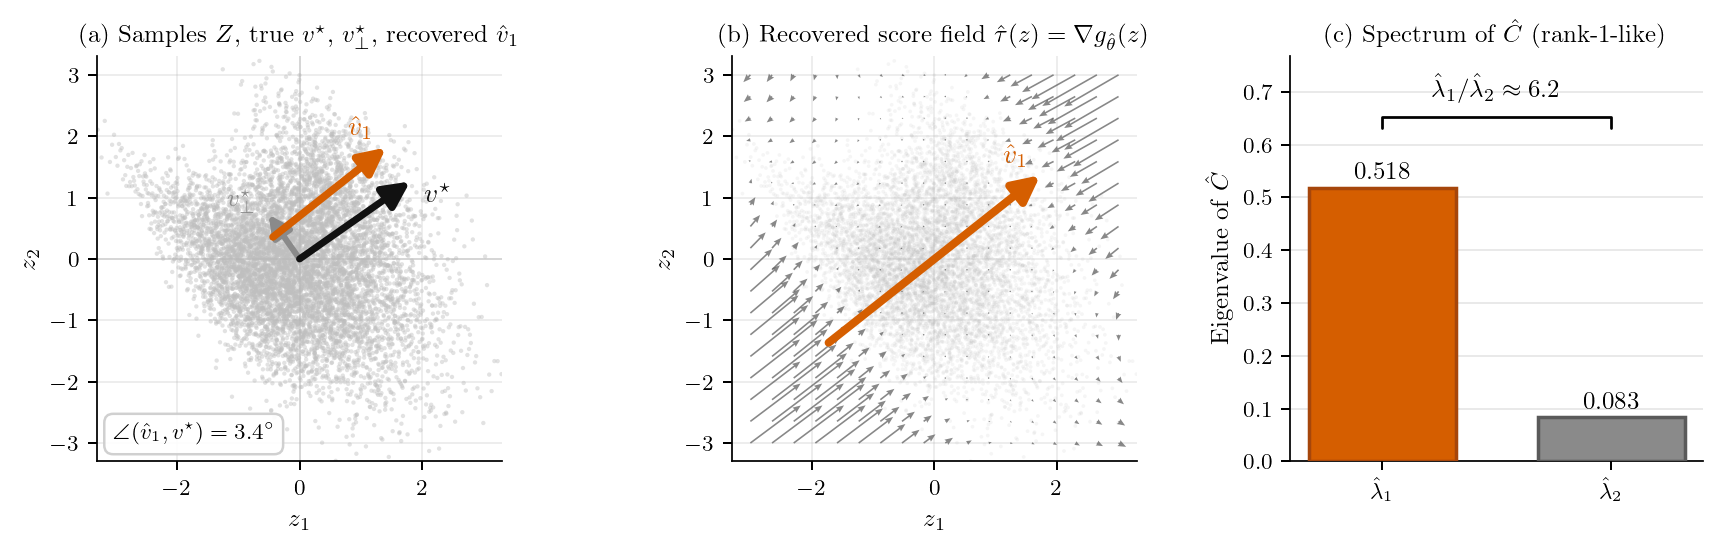
\includegraphics[width=\textwidth]{pedagogical_2d.png}
\caption{\textsc{Cas} is illustrated in two dimensions on a non-Gaussian law whose dependence is concentrated along one non-axis-aligned direction $\vv^\star$, with quadratic conditional-mean dependence. Panel~(a) shows the samples and the top eigenvector $\widehat{\vv}_1$ of $\hmC$, panel~(b) the estimated score field, and panel~(c) the spectrum of $\hmC$.}
\label{fig:pedagogical}
\end{figure}

\paragraph{Hermite polynomial expansion of the log-copula}
Let $h_n$ be the normalized univariate Hermite polynomials ($\EE_{\gauss_1}[h_m h_n] = \delta_{mn}$), $H_\alpha(\vz) := \prod_i h_{\alpha_i}(z_i)$ the tensor basis (orthonormal in $L^2(\gauss_d)$ \cite{Szego1939, Janson1997gaussian}), and
\begin{equation}
  \Lambda_{K,q} \,:=\, \{ \alpha \in \NN_0^d : 1 \leq |\alpha|_1 \leq K,\ |\alpha|_0 \leq q,\ \alpha \neq e_i \text{ for all } i\}
  \label{eq:dict}
\end{equation}
the multi-index set of multivariate Hermite polynomials, whose elements $\alpha$ index the log-copula coefficients $\theta_\alpha$, with maximum total degree $K$ and maximum interaction order $q \leq K$. For Stage 1 we use $\Lambda := \Lambda_{K_1, q_1}$.\footnote{Linear modes $e_i$ are omitted as a modeling choice: a pure linear tilt only re-parametrizes the reference, $e^{\delta z_i}\gauss_d(\vz) = e^{\delta^2/2}\gauss_d(\vz - \delta e_i)$ exactly, though within a nonlinear expansion the omission restricts the dictionary.} The truncation orders $(K_1, q_1)$ and the analogous Stage-2 parameters $(K_2, q_2)$ are chosen for each estimate by cross-validation \cite[\S 7.10]{HastieTibshiraniFriedman2009}, minimizing the score-matching objective on validation samples, the criterion that also chooses the regularizer constants (\Cref{sec:ridge}).\footnote{Supplement~\ref{S-sm:adaptivity} describes an optional greedy choice of the Stage-1 degree and interaction order, with reuse of the score-matching quadratic system.}

Writing $\scL(\vz;\vtheta) := \sum_{\alpha \in \Lambda} \theta^{d}_\alpha H_\alpha(\vz)$ for the parametric log-copula factor and $\scS(\vz;\vtheta) := \nabla\scL(\vz;\vtheta)$ for its gradient, the associated unnormalized Lebesgue density is $\pi_{\vZ}(\vz;\vtheta) := e^{\scL(\vz;\vtheta)}\gauss_d(\vz)$, with \emph{$\vz$-density score}
\begin{equation}
  \nabla\log\pi_{\vZ}(\vz;\vtheta) \;=\; \scS(\vz;\vtheta) - \vz,
  \label{eq:hermite-expansion}
\end{equation}
where the $-\vz$ is the Gaussian-reference score $\nabla\log\gauss_d$.

\paragraph{Hermite copula score matching}
Score matching \cite{Hyvarinen2005} determines $\vtheta$ by minimizing the Fisher divergence between the model $\vz$-density score $\nabla\log\pi_{\vZ}(\cdot;\vtheta)$ and the true score $\nabla\log\pi_{\vZ}$. Because $\scL(\cdot;\vtheta)$ is linear in $\vtheta$, the Hyvärinen identity reduces this to a single linear system $\widehat\mA\,\whvtheta = \widehat\mb$ whose entries are sample averages of Hermite-polynomial derivatives over $\{\vZ^{(n)}\}_{n=1}^N$, assembled by evaluating the expansion and its first two derivatives at the samples with no model simulation and no inner optimization loop. We regularize the inversion with a Tikhonov term \cite{EnglHankeNeubauer1996} and solve
\begin{equation}
  \whvtheta \;=\; (\widehat\mA + \mR_{H^2})^{-1}\widehat\mb, \qquad \mR_{H^2} = \kappa\,\|\widehat\mA\|_{\rm op}\,\diag(|\alpha|_1^2)_{\alpha\in\Lambda}, \quad \kappa = 10^{-4}.
  \label{eq:tikhonov}
\end{equation}
The score-matching identity, the closed forms of $\widehat\mA,\widehat\mb$, and the derivative recurrence behind them are collected in \Cref{app:stage2-foundations} as Hermite copula score matching (HCSM, \Cref{alg:hsm}): a procedure that estimates, from $\vz$-coordinate samples, the Hermite expansion of a copula log-density and hence its score. Stage 2 (\Cref{sec:reduced-model}) applies HCSM to the projected samples.

\paragraph{\textsc{Cas} subspace estimator}
From the coefficients $\whvtheta$, the analytical copula score is $\widehat\scS(\vz) := \nabla\scL(\vz;\whvtheta)$; the score matrix is $\mS \in \RR^{N \times d}$, $\mS_{n,:} = \widehat\scS(\vZ^{(n)})^\top$; and the empirical score second-moment matrix is
\begin{equation}
  \hmC \;:=\; \tfrac{1}{N}\,\mS^\top\mS \;=\; \tfrac{1}{N}\sum_{n=1}^N \widehat\scS(\vZ^{(n)})\,\widehat\scS(\vZ^{(n)})^\top,
  \label{eq:Chat-def}
\end{equation}
with eigenpairs $(\widehat\lambda_i, \widehat\vv_i)_{i=1}^d$ ordered $\widehat\lambda_1 \geq \cdots \geq \widehat\lambda_d$. The top-$r$ eigenvectors form $\hmV_r^{\mC} := [\widehat\vv_1 \;\cdots\; \widehat\vv_r] \in \St(r,\RR^d)$, whose column space is the estimated Stage-1 subspace. \Cref{alg:cas} summarizes the procedure.

\begin{algorithm}[h]
\caption{\textsc{Cas} Stage 1 (subspace identification).}
\label{alg:cas}
\small
\begin{algorithmic}[1]
\Require samples $\{\vn^{(k)}\}_{k=1}^N \subset \RR^d$; maximum total degree $K_1$; maximum interaction order $q_1 \leq K_1$; rank $r$; Tikhonov scale $\kappa \geq 0$; oversampling $p$.
\Ensure eigenbasis $\hmV_r^{\mC} \in \St(r,\RR^d)$ spanning the rank-$r$ subspace, top-$r$ eigenvalues $\widehat\lambda_{1:r}$, stored marginal CDFs $\{\widehat F_i\}_{i=1}^d$, coefficient estimate $\whvtheta$, and tail sum $\widehat E_r$.

\State \textbf{Empirical ranks} $\{\widehat F_i\}_{i=1}^d$ from marginals of $\{\vn^{(k)}\}$; rank-Gaussianize $Z_i^{(k)} = \Phi^{-1}(\widehat F_i(\vn_i^{(k)}))$ per \eqref{eq:rank-transform}, using $\widehat F_i(\vn_i^{(k)}) = R_i^{(k)}/(N+1)$ to avoid the tail blow-up of $\Phi^{-1}$. $\triangleright\ O(Nd\log N)$.

\State \textbf{Enumerate} multi-index set $\Lambda \subset \NN_0^d$ by maximum-degree and interaction-order limits $(K_1, q_1)$ per \eqref{eq:dict}.

\State \textbf{Run HCSM} (\Cref{alg:hsm}) on $\{\vZ^{(k)}\}_{k=1}^N$ with multi-index set $\Lambda$ and regularizer $\mR_{H^2}$, $\to \whvtheta \in \RR^{|\Lambda|}$.

\State \textbf{Assemble score matrix} $\mS \in \RR^{N \times d}$: $\mS_{ki} = \scS_{\whvtheta}(\vZ^{(k)})_i$.

\State \textbf{Extract eigenbasis} $(\hmV_r^{\mC}, \widehat\lambda_{1:r}) \gets $ top-$r$ eigenpairs of $\hmC := \mS^\top\mS / N \in \RR^{d\times d}$ via randomized range-finder \cite{HalkoMartinssonTropp2011} applied to $\mS^\top$ with oversampling $p$; $\hmC$ is never assembled. $\triangleright\ O(Nd(r+p))$.

\State \textbf{Tail sum} $\widehat E_r = \tr(\hmC) - \sum_{i\le r}\widehat\lambda_i = \|\mS\|_F^2/N - \sum_{i\le r}\widehat\lambda_i$ as a finite-sample diagnostic, computable in $O(Nd)$ from $\mS$ without forming further eigenvectors. The optional dictionary search of Supplement~\ref{S-sm:adaptivity} reuses quadratic blocks and a Cholesky factorization under a penalty fixed during the search.
\end{algorithmic}
\end{algorithm}


\subsection{Stage 2: score matching for the reduced density}
\label{sec:reduced-model}

The basis $\hmV_r^{\mC}$ of Stage~1 does not depend on how $c_r^{U}$ is estimated afterwards. On the same subspace, the Hermite estimator below can therefore be replaced by another estimator of $c_r^{U}$ or of its score, such as neural-network score ratio matching \cite{BaptistaBrennanMarzouk2025} or a normalizing flow \cite{PapamakariosEtAl2021}, when an adaptive polynomial approximation in $r$ dimensions is unavailable or inaccurate. Stage~1 still identifies the subspace by a linear score-matching solve and an eigendecomposition. We use Hermite score matching in both stages, which gives $\widehat\scL_r$ and its gradient in closed form.

Stage 2 estimates the reduced factor $c_r^{U}$ on the projected coordinates $\vU = \hmV_r^{\mC\top} \vZ$ by Hermite copula score matching on $\RR^r$. The reduced score $\nabla\scL_r(\vu) = \nabla\log c_r^{U}(\vu)$ relates to the density score by $\partial_j\scL_r(\vu) = \partial_j\log\pi_{\vU}(\vu) + u_j$ since $\pi_{\vU} = c_r^{U}\,\gauss_r$. We use the multi-index set $\Lambda_r := \Lambda_{K_2, q_2}\subset \NN_0^r$ from \eqref{eq:dict}, again excluding constant and linear modes (the reference-mean reparametrization of \Cref{sec:method-core}),\footnote{The second-order modes $H_{2e_j} \in \Lambda_r$ are retained, and represent variance mismatch between $\pi_{\vU}$ and $\gauss_r$.} and parametrize $\log c_r^{U}$ as $\scL_r(\vu;\vbeta) := \sum_{\alpha \in \Lambda_r}\theta^{r}_\alpha H_\alpha(\vu)$, with $\vbeta = (\theta^r_\alpha)_{\alpha\in\Lambda_r}$.

Stage 2 minimizes the Fisher divergence
\begin{equation}
  J(\vbeta)
  \;:=\;
  \tfrac{1}{2}\sum_{j=1}^r\,\EE_{\pi_{\vU}}\!\left[\bigl(\partial_j\scL_r(\vU;\vbeta)-\partial_j\scL_r(\vU)\bigr)^2\right]
  \label{eq:JW-pop}
\end{equation}
between the model and the true reduced scores. By the Hyvärinen identity \cite[Thm.~1]{Hyvarinen2005}, this is again a quadratic in $\vbeta$ \cite[\S4]{Hyvarinen2007}, so Stage 2 is HCSM (\Cref{alg:hsm}) applied to the projected samples $\vu^{(n)} := \hmV_r^{\mC\top}\vZ^{(n)}$ with $d \to r$ and $\Lambda \to \Lambda_r$, assembling the Gram matrix and right-hand side $\widehat\mA_r, \widehat\mb_r$ of \eqref{eq:A-b-formulas}. \Cref{lem:hyv-sm} states the identity and verifies its integration-by-parts hypotheses under Assumption~\ref{ass:tempered}. That quadratic is not minimized freely: \Cref{sec:ridge} states the regularizer and the two constraints it is minimized under, and gives the resulting estimator.

\subsection{Stage-2 regularization and constraints}
\label{sec:ridge}

The unregularized normal equations $\widehat\mA_r\hvbeta = \widehat\mb_r$ are ill-conditioned when the smallest eigenvalues of $\widehat\mA_r$ fall below their sampling error, which is of order $N^{-1/2}$. The penalty restores well-posedness, in the sense of the penalized score-matching estimator of \cite{Sriperumbudur2017}, and its two terms control that estimator's two error sources, the variance from the small eigenvalues and the truncation residual propagated through $\widehat\mA_r^{-1}$.

\subsubsection{The regularizer}
\label{sec:ridge-reg}

\paragraph{Form}
The regularizer is the diagonal, data-driven matrix
\begin{equation}
  \mR(\widehat\mA_r) \;:=\; \underbrace{C_{\rm samp}\,\diag_k\!\bigl(\widehat\sigma_k^2\,\mI_{p_k}\bigr)}_{\mR_{\rm samp}} \;+\; \underbrace{C_{\rm curv}\,\|\widehat\mA_r\|_{\rm op}\,\diag(|\alpha|_1^2)}_{\mR_{\rm curv}},
  \label{eq:R-combined}
\end{equation}
summed over the blocks $\Lambda^{(k)} := \{\alpha\in\Lambda_r:|\alpha|_1 = k\}$ of multi-indices with total degree $k$, with $p_k := |\Lambda^{(k)}|$ and per-degree energy scale $\widehat\sigma_k^2 := \tfrac{1}{N}\tr(\widehat\mA_r^{(k,k)})$, equal to $k\,p_k/N$ under the Gaussian reference. The $|\alpha|_1^2$ weighting is the squared spectral weight of the Ornstein--Uhlenbeck generator on degree-$k$ Hermite polynomials, a Gaussian Sobolev (curvature) penalty \cite{EnglHankeNeubauer1996}.

The two terms damp the directions of the smallest eigenvalues in complementary ways. $\mR_{\rm samp}$ scales with $\widehat\sigma_k^2$, of order $1/N$, so it decreases as $N$ grows. $\mR_{\rm curv}$ scales with $\|\widehat\mA_r\|_{\rm op}$ and the squared degree $|\alpha|_1^2$, is asymptotically $N$-independent, and falls hardest on the high-degree coefficients. Together they keep the solve well-posed at every sample size studied, $N \in [10^2, 10^5]$.

\paragraph{Conditioning} On each block $\Lambda^{(k)}$, $\mR_{\rm curv}$ adds a positive multiple of the identity, which bounds the condition number of that block of $\widehat\mA_r + \mR$ by $1 + 1/(C_{\rm curv}k^2)$ and bounds the whole matrix away from singularity, $\widehat\mA_r + \mR \succeq \min_k(C_{\rm samp}\widehat\sigma_k^2 + C_{\rm curv}\|\widehat\mA_r\|_{\rm op}k^2)\,\mI$.

\paragraph{Choice of the two constants} The two constants $(C_{\rm samp}, C_{\rm curv})$ are chosen for each problem by cross-validation, minimizing the score-matching objective on validation samples, which in fixed coordinates estimates the reduced Fisher divergence \eqref{eq:JW-pop} up to a constant and requires no reference density and no noise model. The choice involves two global scalars, one per term, and both terms are active at every $N \in [10^2, 10^5]$. Supplement~\ref{S-sm:s2reg-empirical} specifies the procedure.

\subsubsection{The two constraints}
\label{sec:ridge-constraints}

\paragraph{Mean-zero score} Alongside the regularizer, we impose the empirical score-mean-zero identity
\begin{equation}
  \widehat\mB\hvbeta = 0,
  \qquad
  \widehat B_{j\alpha} := \tfrac{1}{N}\sum_n \partial_j H_\alpha(\vu^{(n)}),
  \label{eq:centering-mat}
\end{equation}
the empirical form of the identity $\EE_{\pi_{\vU}}[\nabla\log c_r^{U}(\vU)] = 0$ (\Cref{app:regularity}), as a linear constraint. \Cref{prop:centering}, stated after the closed form in \Cref{sec:ridge-solve}, records its effect.

\paragraph{Normalizability} The second constraint makes the reduced factor a probability density with respect to $\gauss_r$. $\scL_r(\cdot;\vbeta)$ is a polynomial, in general unbounded above on $\RR^r$, and without a further constraint $e^{\scL_r}$ need not be integrable against $\gauss_r$. We therefore impose two linear inequality families on $\vbeta$, a level bound $\scL_r(\vu;\vbeta) \le \tau$ on a ball containing the data, for a level $\tau$ computed from the data in \Cref{sec:ridge-solve}, and a strict negativity margin on the leading form of $\scL_r$ over the unit sphere (\Cref{app:solver}). Together they bound $\scL_r$ above on all of $\RR^r$, so $e^{\scL_r}$ is integrable against $\gauss_r$ and $e^{\widehat\scL_r}/\widehat Z_r$ is a probability density with respect to $\gauss_r$.

\subsubsection{The estimator and its solve}
\label{sec:ridge-solve}

The estimator solves
\begin{equation}
\begin{gathered}
  \hvbeta = \arg\min_{\vbeta\,\in\,\mathcal C}\;\tfrac{1}{2}{\vbeta}^\top\bigl(\widehat\mA_r + \mR(\widehat\mA_r)\bigr)\vbeta - {\vbeta}^\top\widehat\mb_r,\\[2pt]
  \mathcal C := \bigl\{\vbeta : \widehat\mB\vbeta = 0,\ \scL_r(\vu;\vbeta) \le \tau \text{ for } \|\vu\| \le r_{\max},\ F[\vbeta](\vv) \le -\varepsilon \text{ for } \|\vv\| = 1\bigr\},
\end{gathered}
  \label{eq:stage2-est}
\end{equation}
with $F[\vbeta]$ the leading form of $\scL_r(\cdot;\vbeta)$ and the radius $r_{\max}$ and margin $\varepsilon$ given in \Cref{app:solver,app:protocol}. The level $\tau$ is computed from the data: the program is first solved with the centering constraint alone, the estimated $\scL_r$ is evaluated at the $N$ samples, and $\tau$ is the $99.9$th percentile of those $N$ values. With the centering constraint alone the solution has the closed form
\begin{equation}
  \hvbeta = \widehat\mM^{-1}\widehat\mb_r - \widehat\mM^{-1}\widehat\mB^\top \bigl(\widehat\mB\widehat\mM^{-1}\widehat\mB^\top\bigr)^{-1}\widehat\mB\widehat\mM^{-1}\widehat\mb_r,
  \quad
  \widehat\mM := \widehat\mA_r + \mR(\widehat\mA_r).
  \label{eq:stage2-closedform}
\end{equation}
The solve requires one Cholesky factorization \cite{GolubVanLoan2013} of the $|\Lambda_r| \times |\Lambda_r|$ matrix $\widehat\mM$ and one $r \times r$ linear solve. The sizes of both matrices depend on the reduced dimension $r$ and not on $d$. With $\hvbeta$ in hand, the gradient of \eqref{eq:cas-estimator} follows by the chain rule through $\widehat\scZ$ wherever the transform is differentiable (\Cref{app:protocol}).

Each inequality in $\mathcal C$ is linear in $\vbeta$ because $\scL_r(\vu;\cdot)$ and $F[\cdot](\vv)$ are linear in the coefficients, so $\mathcal C$ is an intersection of half-spaces, hence convex, indexed by the points of the ball and the sphere. The solver imposes the two families at a finite set of points, enlarged iteratively by the points at which a search over the ball and the sphere finds the largest violation, until the search finds none beyond its tolerance or a round limit is reached (\Cref{app:solver}). Each re-solve is a convex quadratic program with the added rows as inequality constraints, and when the solution of \eqref{eq:stage2-closedform} already satisfies both families at every searched point, no points are added and the estimator equals \eqref{eq:stage2-closedform}.

The centering constraint changes both the bias and the variance of the solve, and the following proposition describes what it does to each.

\begin{proposition}[Properties of the centering constraint]
\label{prop:centering}
Fix the true rank transform, a deterministic basis, the multi-index set $\Lambda_r$, and the regularizer $\mR$, so that the projected sample is i.i.d. Let $\hvbeta$ be the centered Stage-2 estimator \eqref{eq:stage2-closedform} and $\hvbeta_{\rm unc} := \widehat\mM^{-1}\widehat\mb_r$ the unconstrained solve. Let $\mA^\star, \mB^\star, \bm b^\star$ be the $N\to\infty$ limits of $\widehat\mA_r, \widehat\mB, \widehat\mb_r$, with $\mB^\star$ of full row rank, set $\bm M := \mA^\star + \mR$, let $\Pi^\star$ be the $\bm M$-orthogonal projector onto $\mathrm{range}(\bm M^{-1}\mB^{\star\top})$, let $\bm\theta^{r,\star}$ be the truncated minimizer $\mA^\star\bm\theta^{r,\star} = \bm b^\star$, and let $\bar{\bm\theta} := (\mI-\Pi^\star)\bm M^{-1}\bm b^\star$ be the centered solve of the limiting system. Then:

\emph{(i) The constraint acts by projection.} $\hvbeta = (\mI - \Pi_{\widehat\mB})\hvbeta_{\rm unc}$, where $\Pi_{\widehat\mB} := \widehat\mM^{-1}\widehat\mB^\top(\widehat\mB\widehat\mM^{-1}\widehat\mB^\top)^{-1}\widehat\mB$ is the $\widehat\mM$-orthogonal projector onto $\mathrm{range}(\widehat\mM^{-1}\widehat\mB^\top)$, defined whenever $\widehat\mB$ has full row rank.

\emph{(ii) It replaces one bias by another.} The centered solve of the limiting system satisfies the exact identity
\begin{equation}
  \bar{\bm\theta} - \bm\theta^{r,\star}
  = \underbrace{-(\mI - \Pi^\star)\,\bm M^{-1}\mR\,\bm\theta^{r,\star}}_{\text{regularization bias, contracted}}
  \;\underbrace{-\; \Pi^\star\bm\theta^{r,\star}}_{\text{truncation bias, added}},
  \label{eq:centering-bias}
\end{equation}
whose first term is the unconstrained regularization bias $-\bm M^{-1}\mR\bm\theta^{r,\star}$ after an $\bm M$-orthogonal contraction that cannot enlarge it ($\|\mI-\Pi^\star\|_{\bm M} \le 1$), and whose second term is $\Pi^\star\bm\theta^{r,\star} = -\bm M^{-1}\mB^{\star\top}(\mB^\star\bm M^{-1}\mB^{\star\top})^{-1}\EE_{\pi_{\vU}}[\bm\rho]$, fixed by $\mB^\star\bm\theta^{r,\star} = -\EE_{\pi_{\vU}}[\bm\rho]$ for the Fisher truncation residual $\bm\rho := \nabla\scL_r - \Pi_{\Lambda_r}\nabla\scL_r$ ($\Pi_{\Lambda_r}$ the $L^2(\pi_{\vU})$ projection onto $\mathrm{span}\{\nabla H_\alpha : \alpha\in\Lambda_r\}$), and equal to zero exactly when $\EE_{\pi_{\vU}}[\bm\rho] = 0$.

\emph{(iii) The limiting projection is non-expansive.} The $\bm M$-orthogonal projection does not increase the $\bm M$-weighted variance: for every random $\bm\xi$ with finite second moment,
\begin{equation}
  \tr\!\bigl(\mA^\star\Cov((\mI-\Pi^\star)\bm\xi)\bigr) \;\le\; \tr\!\bigl(\bm M\,\Cov(\bm\xi)\bigr).
  \label{eq:centering-var}
\end{equation}

\emph{(iv) The estimator reaches $\bar{\bm\theta}$ at the Monte Carlo rate.} Under \Cref{ass:tempered} the sample averages $(\widehat\mB, \widehat\mM, \widehat\mb_r)$ obey a central limit theorem, so $\|\hvbeta - \bar{\bm\theta}\| = O_p(N^{-1/2})$.
\end{proposition}

\emph{Proof.} See \Cref{app:centering}.

The regularization bias of \eqref{eq:centering-bias} carries the factor $\mR$; its sampling-noise part decreases with $N$ through the term $\mR_{\rm samp} \asymp 1/N$ of \eqref{eq:R-combined}, its curvature part need not, and the truncation bias is $N$-independent and equals zero when the reduced score is representable in $\Lambda_r$. The sign of the net effect therefore depends on the problem and on $N$, and Supplement~\ref{S-sec:sm2-centering} measures it on Examples~1--3.

\paragraph{Independence of the basis} Stage 1 identifies a subspace, and any orthonormal basis of that subspace could be handed to Stage 2, so the Stage-2 estimate should not depend on which basis is used. When the specified maximum interaction order excludes no multi-index ($q_2 \ge \min(K_2, r)$, in which case the condition $|\alpha|_0 \le q_2$ removes nothing from $\Lambda_r$), the estimator with exact optimization and integration is invariant. A basis change $\hmV_r^{\mC} \mapsto \hmV_r^{\mC}\mQ$ with $\mQ \in \mathrm{O}(r)$ rotates the coordinates $\vu$, and a rotation maps the span of the Hermite polynomials of each total degree $k$ onto itself. Every quantity in the solve is then unchanged or transforms consistently: the span of the model polynomials, the per-degree scales $\widehat\sigma_k^2$, and $\|\widehat\mA_r\|_{\rm op}$ are unchanged; the regularizer $\mR$, which multiplies all coefficients of the same total degree by one scalar, commutes with the rotation; the centering constraint set $\{\vbeta : \widehat\mB\vbeta = 0\}$ maps onto itself; and the estimated density $\widehat\pi_{\vn}$ is unchanged. When the maximum interaction order excludes multi-indices ($q_2 < K_2$ and $q_2 < r$), the estimate depends on the basis through the excluded multi-indices; the numerical search and quadrature of \Cref{app:solver,app:protocol} are not rotated with the basis.

\paragraph{Performance of the chosen constants}
The chosen constants stay within $0.18$ nats in held-out log-score of the best alternative regularizer on all three examples of \Cref{sec:experiments} at every $N \in [10^2, 10^5]$, while the unregularized solve raises that score by $2.8$--$3.6$ nats at $N = 100$. On the inference problem of \Cref{sec:exp-bip}, the proposed estimator is within $0.04$ nats in posterior KL divergence of the Tikhonov regularizer $\mR_{H^2}$ of \eqref{eq:tikhonov} applied to $\widehat\mA_r$ at the best $\kappa$ chosen separately for each $N$. That best $\kappa$ shifts from $3\times10^{-2}$ at $N = 10^2$ to $10^{-5}$ at $N = 5\times10^4$, so no single $\kappa$ on the grid matches it. Supplement~\ref{S-sm:s2reg-empirical} reports the comparison in full.

% =====================================================================
\section{Error at the estimated Stage-1 subspace}
\label{sec:theory}

\Cref{thm:kl-trunc} holds for every $\mV_r \in \St(r,\RR^d)$, in particular at the estimated Stage-1 subspace $\hmV_r^{\mC}$ of \Cref{sec:method-core}: $\DKL\bigl(\pi_{\vn}\,\|\,\pi_{\vn}(\,\cdot\,;\hmV_r^{\mC})\bigr) \le \tfrac12\tr\bigl((\mI-\hmP_r)\mC\bigr)$, where $\hmP_r := \hmV_r^{\mC}\hmV_r^{\mC\top}$. The trace is not computable from the samples, because $\mC$ is the covariance of the unknown copula score. \Cref{prop:diagnostic} makes two statements about the matrix $\mC_\Lambda$ of Stage 1, defined below: the trace at the estimated subspace exceeds its minimum by at most a quadratic in the recovery angle, so the excess is second order in that angle, and the tail sum $\widehat E_r$ of \Cref{alg:cas} estimates that minimum, with a bound on the error of the estimate.

We introduce the following objects, all of which appear in \Cref{prop:diagnostic}. The \emph{parameterized score} $\scS_\Lambda$ is the $L^2(\pi_{\vZ})$ orthogonal projection of the true copula score $\scS$ onto the Hermite score field $\scF_\Lambda := \{\sum_{\alpha\in\Lambda}\theta_\alpha\nabla H_\alpha\}$ over the Stage-1 multi-index set $\Lambda$ of \eqref{eq:dict}, $\mC_\Lambda := \EE_{\pi_{\vZ}}[\scS_\Lambda(\vZ)\,\scS_\Lambda(\vZ)^\top]$ is its second-moment matrix, and the \emph{Hermite truncation error} $\|\scS - \scS_\Lambda\|_{L^2(\pi_{\vZ})}$ does not increase as $\Lambda$ grows. Two rank-$r$ subspaces appear below: the \emph{projection subspace} $\mV_{r,\Lambda}$, the leading rank-$r$ eigenspace of $\mC_\Lambda$, and the \emph{estimated Stage-1 subspace} $\hmV_r^{\mC}$, which Stage 1 returns from $N$ samples. The Stage-1 solve carries the fixed penalty of \eqref{eq:tikhonov}, so $\mV_{r,\Lambda}$ is a benchmark for $\hmV_r^{\mC}$ rather than its limit. Neither is the bound-optimal $\mV_r^{\mC}$ of \Cref{cor:optimal-subspace}, the leading rank-$r$ eigenspace of the true score covariance $\mC$. The angle $\|\sin\Theta(\mV_{r,\Lambda}, \mV_r^{\mC})\|_F$ between $\mV_{r,\Lambda}$ and $\mV_r^{\mC}$ is induced by the Hermite truncation alone. Write $\mP_{r,\Lambda} := \mV_{r,\Lambda}\mV_{r,\Lambda}^\top$, and $E_r(\mC_\Lambda) := \sum_{i>r}\lambda_i(\mC_\Lambda) = \tr((\mI-\mP_{r,\Lambda})\mC_\Lambda)$, the sum of the eigenvalues of $\mC_\Lambda$ below the retained rank, for the \emph{rank-$r$ truncation error of $\mC_\Lambda$}.

\begin{proposition}[Rank-$r$ truncation error and its diagnostic]
\label{prop:diagnostic}
For $1 \le r < d$, let $\|\sin\Theta\|_F := \|\sin\Theta(\hmV_r^{\mC}, \mV_{r,\Lambda})\|_F$ be the principal-angle distance between the estimated Stage-1 subspace and the projection subspace. Over rank-$r$ orthogonal projectors $\mP$, the trace $\tr((\mI-\mP)\mC_\Lambda)$ is smallest at $\mP_{r,\Lambda}$, where it equals $E_r(\mC_\Lambda)$; at the estimated Stage-1 subspace it exceeds this minimum by $\tr((\mI-\hmP_r)\mC_\Lambda) - E_r(\mC_\Lambda) = \tr((\mP_{r,\Lambda}-\hmP_r)\mC_\Lambda) \ge 0$, bounded above and below by quadratics in $\|\sin\Theta\|_F$,
\begin{equation}
  (\lambda_r-\lambda_{r+1})(\mC_\Lambda)\,\|\sin\Theta\|_F^2
  \;\le\;
  \tr\bigl((\mP_{r,\Lambda}-\hmP_r)\,\mC_\Lambda\bigr)
  \;\le\;
  (\lambda_1-\lambda_d)(\mC_\Lambda)\,\|\sin\Theta\|_F^2,
  \label{eq:misalign-quadratic}
\end{equation}
and the sample tail sum $\widehat E_r := \sum_{i>r}\widehat\lambda_i$ of the eigenvalues of $\hmC$ estimates the rank-$r$ truncation error of $\mC_\Lambda$ with
\begin{equation}
  \bigl|\widehat E_r - E_r(\mC_\Lambda)\bigr| \;\le\; \sum_{j=1}^{d-r}\sigma_j\bigl(\hmC - \mC_\Lambda\bigr) \;\le\; (d-r)\,\|\hmC - \mC_\Lambda\|_{\rm op},
  \label{eq:Ehat-weyl}
\end{equation}
where $\sigma_1(\cdot) \ge \cdots \ge \sigma_d(\cdot)$ denote singular values in decreasing order.
\end{proposition}

\emph{Proof.} See \Cref{app:thm-trunc}.

This excess is quadratic in the recovery angle $\|\sin\Theta\|_F$, so an approximate subspace suffices. The rank-$r$ truncation error of $\mC_\Lambda$ is not a sampling error and depends only on the retained rank, decreasing with larger $r$, and the tail sum $\widehat E_r$ estimates it from the samples alone (\Cref{alg:cas}, step~6), with \eqref{eq:Ehat-weyl} bounding the error of that estimate by the leading singular values of $\hmC - \mC_\Lambda$. The difference between the quantities of $\mC_\Lambda$ and their counterparts at the true $\mC$ is induced by the Hermite truncation error and is not quantified here (\Cref{sec:limitations}). That truncation error need not be small for the subspace to be identified (\Cref{lem:pilot-subspace}).

\begin{lemma}[Identification under exact rank-$r$ dependence]
\label{lem:pilot-subspace}
Let $\pi_{\vZ}$ satisfy \Cref{ass:tempered} and suppose the dependence is exactly rank $r$: $c^{Z}(\vz) = c_r^{U}(\mV_r^\top\vz)$ for some $\mV_r \in \RR^{d\times r}$ with $\mV_r^\top\mV_r = \mI_r$, equivalently $\pi_{\vZ} = \pi_{\vU}\otimes\gauss_{d-r}$ in the coordinates $\vu = \mV_r^\top\vz$, $\vw = \mV_\perp^\top\vz$ of \Cref{sec:reduced-form}. Fix $K \geq 2$ and let $\Lambda_{K,d}$ be the index set of \eqref{eq:dict} with no maximum interaction order imposed (any $q \geq K$, since $|\alpha|_0 \le |\alpha|_1$), so that $\Lambda_{K,d} = \{\alpha \in \NN_0^d : 2 \le |\alpha|_1 \le K\}$, and let $\scS_\Lambda$ be the infinite-sample score-matching solution over $\Lambda_{K,d}$, the minimizer of $\EE_{\pi_{\vZ}}[\|\sum_{\alpha}\theta_\alpha\nabla H_\alpha - \scS\|^2]$. Then $\scS_\Lambda(\vz) \in \mathrm{span}(\mV_r)$ for every $\vz$, and $\scS_\Lambda$ depends on $\vz$ only through $\vu$. Consequently $\mC_\Lambda = \mV_r\,\mathbf M\,\mV_r^\top$ for a positive semidefinite $\mathbf M \in \RR^{r\times r}$, and whenever $\mC_\Lambda$ attains rank $r$ its top-$r$ eigenspace equals $\mathrm{span}(\mV_r)$, for any value of $\|\scS - \scS_\Lambda\|_{L^2(\pi_{\vZ})}$.
\end{lemma}

\emph{Proof.} See \Cref{app:pilot-subspace}.

\begin{remark}[Identifying the active subspace with a coarse Stage-1 Hermite expansion]
\label{rem:pilot-subspace}
\Cref{lem:pilot-subspace} separates two requirements that are easily conflated. Representing the copula score accurately requires a $\Lambda$ rich enough to make $\|\scS - \scS_\Lambda\|_{L^2(\pi_{\vZ})}$ small. Identifying the active subspace does not.

Under exact rank-$r$ dependence, every eigenvector of $\mC_\Lambda$ with a nonzero eigenvalue lies in the active subspace at every $K \geq 2$, so a coarse $\Lambda$ can miss active directions but cannot introduce complement ones. The top-$r$ eigenspace equals the active subspace as soon as $\scS_\Lambda$ has a nonzero component along every active direction, which is the rank-$r$ condition of the lemma. The expansion that must represent a score is the Stage-2 one, in $r$ variables rather than $d$.

The conclusion concerns the span at a known $r$ and not the eigenvalue ordering. Truncation reweights the nonzero eigenvalues, so the lemma supports recovery at known $r$ rather than the choice of $r$ by an eigenvalue threshold.

Two features of the estimator depart from the lemma's idealization, the maximum interaction order $q_1 < K_1$, which can introduce components outside the active subspace, and imperfect rank-$r$ concentration, and \Cref{sec:exp-banana} measures the resulting deviation against the reference $\mV_r^{\mC}$ (\Cref{fig:recovery-row}).
\end{remark}

% =====================================================================
\section{Experiments}
\label{sec:experiments}

\paragraph{Methods} Four noise estimators are compared: (i) the product of marginals (PoM), the independence assumption of univariate noise modeling; (ii) the Gaussian copula, which admits arbitrary marginals but represents dependence only through a correlation matrix; (iii) PCA-HCSM, which shares the full \textsc{Cas} procedure but chooses its rank-$r$ subspace by variance; and (iv) \textsc{Cas}, the rank-$r$ score-covariance subspace with Hermite copula score matching on the projection. The first three are the common simplifications of \Cref{sec:intro}, and the gap from each to \textsc{Cas} measures what the score-covariance subspace adds over that simplification.

The experiments measure three quantities on three example problems, defined next. Subspace recovery comes first, then noise KL divergence, then posterior KL divergence in a Bayesian inference problem. Only (iii) and (iv) choose a rank-$r$ subspace, so only those two enter the subspace-recovery comparison, while all four enter the density and posterior comparisons. \Cref{thm:kl-trunc} bounds the part of the second quantity that the first controls, the divergence of the reduction at a given subspace, and \eqref{eq:posterior-noise-kl} bounds the third by the second. We report results against the number of samples $N$, over $N \in \{500, 1000, 2000, 5000, 10000, 20000, 50000\}$, with the numbers quoted in the text taken at the largest, $N = 50{,}000$. Per-example diagnostics and the sweep over reduced rank $r$ are reported in Supplement~\ref{S-sm:rate-real}.

\subsection{Example problems}
\label{sec:exp-benchmark}

All three examples share one construction and differ only in the map that creates the dependence. Let $\vW \in \RR^{20}$ have independent standard Gaussian coordinates. In each example two of the first four coordinates are replaced by bounded nonlinear functions of the other two, each perturbed by independent Gaussian noise: in Examples~1 and~3 the pair $(W_0, W_1)$ determines the pair $(W_2, W_3)$, and in Example~2 there are two separate input--output pairs, $W_0$ determining $W_1$ and $W_2$ determining $W_3$. Each replaced coordinate is rescaled so that $\EE[W_j] = 0$ and $\Var(W_j) = 1$ for every $j$, and the remaining $16$ coordinates are left as independent standard Gaussians. Four latent coordinates therefore carry dependence, $r^\star = 4$. The latent vector is then mixed by a uniformly random rotation $\mQ \sim \mathrm{Unif}(\mathrm{O}(8))$, drawn from the Haar probability measure on the orthogonal group, acting on the first $8$ coordinates and as the identity on the remaining $12$, so that the four dependent directions are not axis-aligned; the componentwise map $n_j = \mathrm{logit}(\Phi(z_j))$ is then applied to $\vz = \mQ\vW$. Because $\mQ$ is orthogonal and $\EE[\vW\vW^\top] = \mI_{20}$, the latent coordinates satisfy $\EE[\vz\vz^\top] = \mI_{20}$, so their covariance does not distinguish the four dependent directions.

In Example~1, the primary example problem, the two outputs are the real and imaginary parts of $(W_0 + iW_1)^2$, saturated by $\tanh$:
\begin{equation}
\begin{gathered}
  W_0, W_1 \sim \gauss(0, 1), \\
  W_2 = c\,\tanh\!\bigl((W_0^2 - W_1^2)/M\bigr) + \sqrt{1 - a^2}\,\varepsilon_2, \\
  W_3 = c\,\tanh\!\bigl(2 W_0 W_1/M\bigr) + \sqrt{1 - a^2}\,\varepsilon_3,
\end{gathered}
  \label{eq:ex1-block}
\end{equation}
with $\varepsilon_2, \varepsilon_3 \sim \gauss(0,1)$, saturation scale $M = 2.5$, conditional-mean variance fraction $a = 0.7$, and amplitude $c$ fixed by $\Var(c\tanh(\cdot)) = a^2$.

In this law the latent pairwise correlations vanish, $\EE[W_iW_j] = 0$ for $i \ne j$, so the dependence it creates is of higher order. Its two-to-one map $z \mapsto z^2$ ($z = W_0 + iW_1$) makes the conditional law of the two input coordinates given the two output coordinates bimodal, symmetric under $z \mapsto -z$, which gives the posterior of \Cref{sec:exp-bip} two branches, so the non-Gaussianity has a visible posterior consequence.

The reference subspace $\mV_r^{\mC}$ of \Cref{cor:optimal-subspace} is the top-$r$ eigenspace of the true score covariance $\mC := \EE_{\vz \sim \pi_{\vZ}}[\nabla \log c^{Z}(\vz)\, \nabla \log c^{Z}(\vz)^\top]$, which has no closed form. Each mixed coordinate has a marginal density given by a Gaussian mixture over the input coordinates, so the copula score $\nabla\log c^{Z}$ can be evaluated directly; we evaluate $\mC$ by Monte Carlo at $N_{\mathrm{ref}} = 10^6$ from that score and take $\mV_r^{\mC}$ to be its top-$r$ eigenspace (Supplement~\ref{S-sm:rate-real}). The reference spectrum has top-$4$ eigenvalues $\approx 2.29, 2.28, 0.95, 0.92$, with the remaining $16$ eigenvalues summing to $\approx 0.04$. The cutoff $r^\star = 4$ equals the number of coupled latent coordinates.

\paragraph{Two further examples} Examples~2 and~3 differ from Example~1 only in the map from inputs to outputs, chosen so that the copula score is harder (Example~2) and easier (Example~3) for a Hermite expansion to represent than Example~1's.

\emph{Example~2.} Each output is an even function of its input: for $j \in \{0, 2\}$, $W_{j+1} = c\,(\tanh(\gamma(W_j^2 - 1)) - m_0) + \sqrt{1 - a^2}\,\varepsilon$ with $\gamma = 0.5$, $a = 0.7$, centering $m_0 = \EE[\tanh(\gamma(W_j^2 - 1))]$, and variance-normalizing $c$. An even map is non-injective, and its copula score is harder for a Hermite expansion to represent, though the score covariance still identifies the active subspace. Its top-$4$ score-covariance eigenvalues are $\approx 2.28, 2.16, 0.95, 0.80$, with the remaining $16$ summing to $\approx 0.09$.

\emph{Example~3.} The two outputs are the real and imaginary parts of $(W_0 + iW_1)^3$: $W_2 = c\,\tanh((W_0^3 - 3 W_0 W_1^2)/M) + \sqrt{1 - a^2}\,\varepsilon_2$ and $W_3 = c\,\tanh((3 W_0^2 W_1 - W_1^3)/M) + \sqrt{1 - a^2}\,\varepsilon_3$, with $M = 4$, $a = 0.7$, $c \approx 1.48$; both output means vanish by symmetry. The score is smooth and the easiest of the three to represent, and the three-to-one map $z \mapsto z^3$ yields a three-modal posterior. Its top-$4$ score-covariance eigenvalues are $\approx 4.42, 4.39, 0.97, 0.94$, with the remaining $16$ summing to $\approx 0.04$.

All three examples appear in every stage of \Cref{sec:exp-banana}--\Cref{sec:exp-bip}, with Example~1 supplying the main reported numbers and the posterior illustration of \Cref{fig:bip-posteriors}.

\subsection{Subspace recovery: score covariance versus PCA}
\label{sec:exp-banana}

The latent covariance does not distinguish the four dependent directions, and this subsection checks that the score covariance finds them and that PCA does not. For $r = r^\star = 4$ we measure each estimate against $\mV_r^{\mC}$ over $20$ independent realizations at each $N$, with the multi-index set of each estimate chosen by cross-validation on its own sample (\Cref{sec:method-core}). The \textsc{Cas} angle decreases with $N$, while the PCA and uniformly random angles are $N$-independent and equal within the across-realization spread (\Cref{fig:recovery-row}, all three examples). The \textsc{Cas} angle also depends on the chosen multi-index set: the cross-validation criterion chooses interaction order $q_1 = 2$ in every realization for $N \le 10{,}000$ and a higher interaction order ($q_1 = 3$ on Examples~1--2, $q_1 = 4$ with even degrees on Example~3) in every realization at $N = 50{,}000$, where the mean angle is smaller than at $N = 10{,}000$ by factors of $16$, $6.0$ and $11$ on Examples~1--3. At $N = 20{,}000$ the higher order is chosen in $11$ and $3$ of the $20$ realizations on Examples~1 and~3, and the band is wider there.

A second comparison removes Stage-2 estimation entirely, evaluating $D_{\mathrm{KL}}(\pi_{\vZ}\,\|\,\pi_{\vZ}(\,\cdot\,;\mV_r))$, the divergence the reduction alone incurs when the reduced density on the subspace is exact: the \textsc{Cas} divergence decreases with $N$ toward its value at the reference $\mV_r^{\mC}$ on all three examples, while the PCA divergence does not decrease and lies within the spread of uniformly random subspaces (Supplement~\ref{S-sec:subspace-only-kl}).

\begin{figure}[t]
\centering
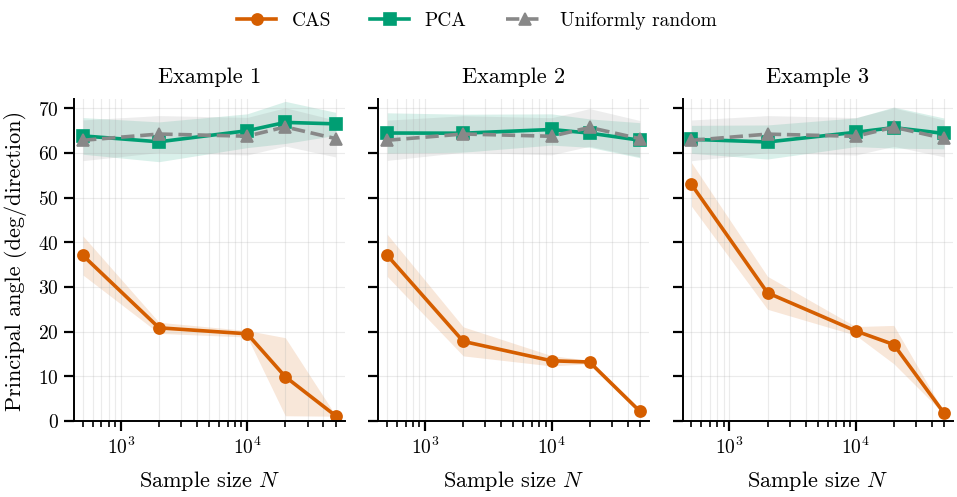
\includegraphics[width=\textwidth]{recovery_row.png}
\caption{Subspace recovery on Examples~1--3 is measured as the per-direction principal angle \cite{BjorckGolub1973} to the bound-optimal subspace $\mV_r^{\mC}$ versus sample size $N$, over $20$ independent realizations with bands of $\pm1$ standard deviation. The \textsc{Cas} angle decreases with $N$ and depends on the chosen multi-index set, while the angles of PCA and of a uniformly random subspace are $N$-independent.}
\label{fig:recovery-row}
\end{figure}

\subsection{Noise KL divergence of the reduced density}
\label{sec:exp-testll}

The rank is $r = r^\star = 4$, and both rank-$r$ methods use the regularizer of \Cref{sec:ridge}. Each method is estimated on a sample of $N$ residuals and evaluated on an independent sample of the same size, over $20$ independent realizations; within a realization all four estimators use the same estimation sample and the same evaluation sample, so the comparison is paired. \textsc{Cas} attains the lowest noise KL divergence (mean $0.128$; \Cref{fig:testll}), versus $0.70$ for PCA-HCSM, $0.70$ for PoM, and $0.70$ for the Gaussian copula. PCA-HCSM and \textsc{Cas} differ only in how the rank-$r$ subspace is chosen, with the Hermite polynomial basis, regularizer, and quasi--Monte Carlo normalizer held fixed, so the gap between them equals the contribution of choosing the subspace by score covariance. At $N = 50{,}000$ the across-realization standard deviation is $0.011$ for \textsc{Cas} and at most $0.009$ for the baselines. The same ordering holds on Examples~2 and~3 (\Cref{fig:testll}): the three baselines converge to a shared noise KL divergence as $N$ grows, the dependence none of them represents, while the \textsc{Cas} divergence continues to decrease and is smaller at the largest $N$. Supplement~\ref{S-sm:rate-real} reports the full sweep over reduced rank $r$.

\begin{figure}[ht]
\centering
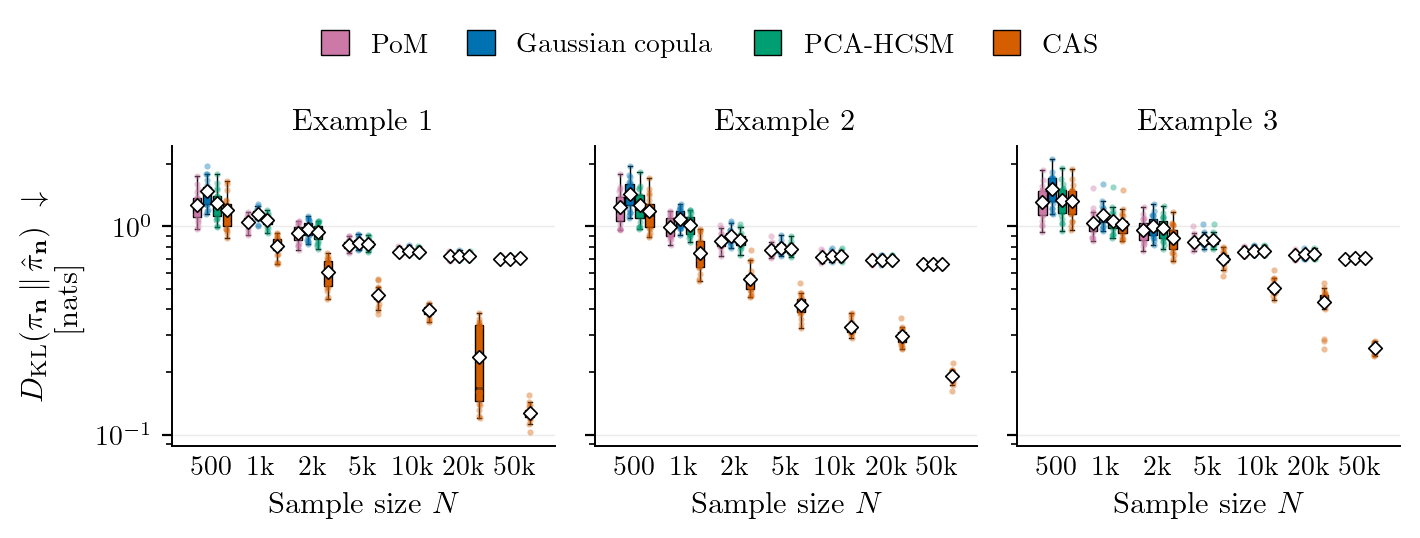
\includegraphics[width=\textwidth]{test_ll_all.png}
\caption{Noise KL divergence on Examples~1--3 is shown for $r=4$ across sample sizes, with $20$ independent realizations at each $N$.}
\label{fig:testll}
\end{figure}

\subsection{Bayesian inference problem with non-Gaussian observation noise}
\label{sec:exp-bip}

We now study the effect of the noise estimator on the posterior. The estimated noise density is used as the likelihood, so an observation $\vy$ contributes $\widehat\pi_{\vn}(\vy - \mA\vx)$, and the question is whether the resulting posterior is closer to the true-noise posterior than the alternatives.

\paragraph{Problem} The parameter dimension is $d_{\mathrm{par}} = 2$, the observation dimension is $d_{\mathrm{obs}} = 20$, and the prior is $\pi_X(\vx) = \gauss(\vx; 0, \sigma_0^2 I_2)$ with $\sigma_0 = 2$. The forward map observes the two input directions of Example~1, the first two columns of $\mQ$, which are orthonormal:
\begin{equation}
  \vy \;=\; \mA \vx + \vn, \qquad \mA \;=\; \alpha\, \mQ_{:,\,0{:}2}, \qquad \alpha = 1.5.
  \label{eq:bip-forward}
\end{equation}
Varying $\vx$ therefore moves the residual along those two directions alone, and the bimodal conditional law of \Cref{sec:exp-benchmark} gives the posterior two branches. We compare the four noise estimators at rank $r = 4$; for each of the $20$ independent realizations at each $N$, every method is estimated on that realization's residual sample and evaluated on one observation $\vy = \mA\vx^{\star} + \vn$. The KL divergence is computed on an $80\times 80$ grid over $[-6, 6]^2$, with each candidate posterior normalized to unit mass on the grid (\Cref{app:protocol}).

\Cref{fig:bip-kl} aggregates posterior KL divergence across all sample sizes. For $N = 50{,}000$, \textsc{Cas} attains mean posterior KL divergence $0.051$, versus $0.40$ for PCA-HCSM, $0.40$ for PoM, and $0.40$ for the Gaussian-copula baseline. At $N = 500$ the four means lie between $0.40$ and $0.49$ nats. \Cref{fig:bip-posteriors} shows the posteriors for one observation at $N=50{,}000$, chosen because it places mass on both preimage branches: the three baselines each produce a single broad mode between the branches, and only \textsc{Cas} places mass on both. The ranking matches the noise KL divergence of \Cref{fig:testll} and the subspace recovery of \Cref{fig:recovery-row}.

\begin{figure}[t]
\centering
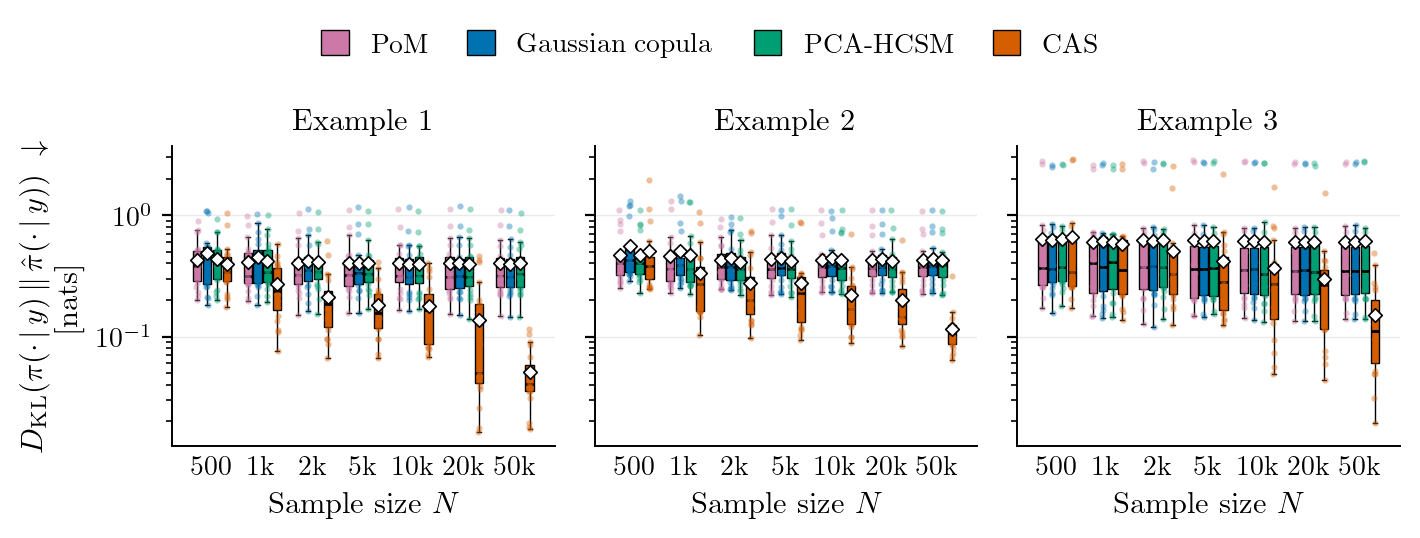
\includegraphics[width=\textwidth]{bip_kl_all.png}
\caption{Posterior KL divergence from the true-noise posterior is shown on Examples~1--3 across $N$ for $r=4$, with $20$ independent realizations at each $N$.}
\label{fig:bip-kl}
\end{figure}

\begin{figure}[t]
\centering
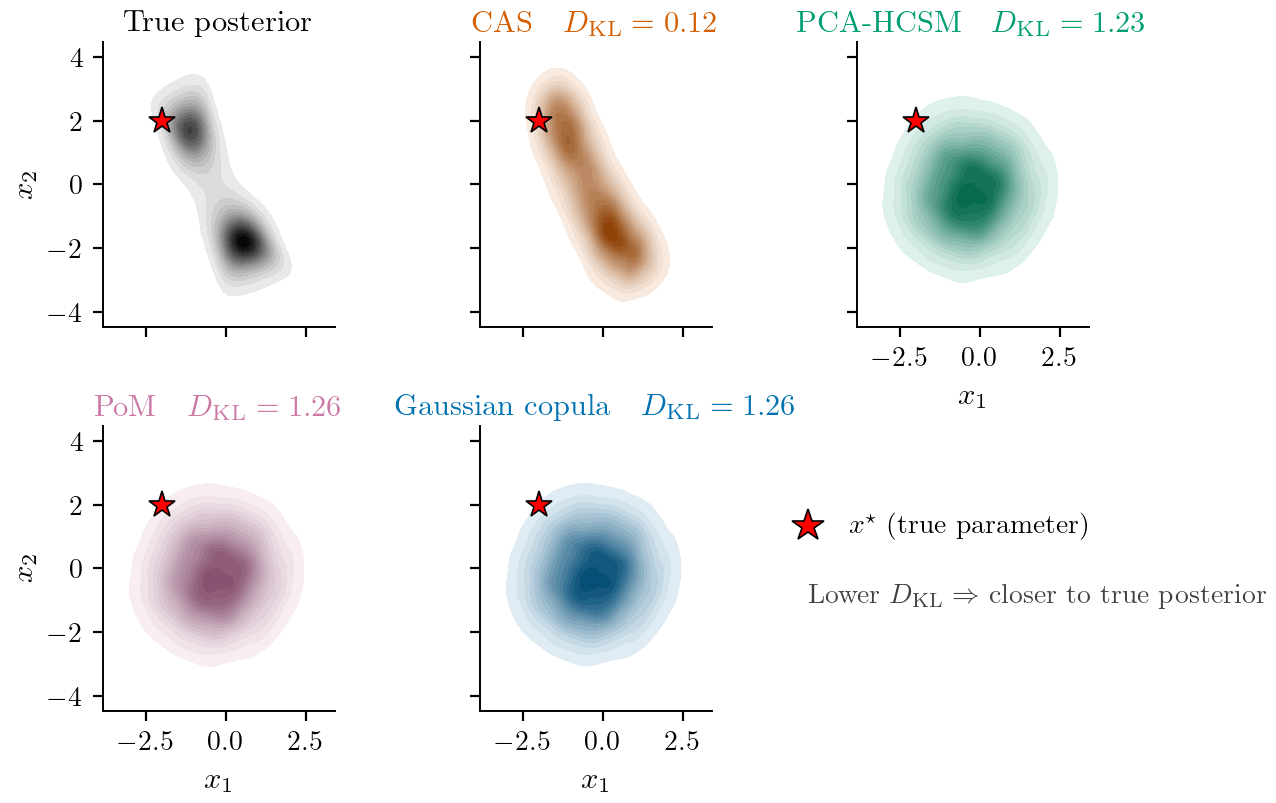
\includegraphics[width=0.85\textwidth]{bip_posteriors.png}
\caption{Posterior shapes are compared for one observation of the inference problem of \Cref{sec:exp-bip} with $N=50{,}000$, for $r=4$, a $20$-dimensional observation, and a $2$-dimensional parameter; the observation is chosen to place mass on both preimage branches, and the divergences shown are those of this observation rather than the means of \Cref{fig:bip-kl}. The true posterior places mass on both branches, and the \textsc{Cas} noise model reproduces both modes, while PCA-HCSM, the product-of-marginals model, and the Gaussian-copula baseline each yield a single broad mode.}
\label{fig:bip-posteriors}
\end{figure}

% =====================================================================
\section{Limitations and scaling}
\label{sec:limitations}

The reduction is linear in $\vZ$-space: dependence that varies along a curved set of directions is retained only through its variation along the chosen subspace, and transport-based reductions \cite{MarzoukMoselhyParnoSpantini2016, BaptistaMarzoukZahm2023representation, BrennanBigoniZahmSpantiniMarzouk2020, ChenArnaudBaptistaZahm2024} are the nonlinear alternatives. Assumption~\ref{ass:tempered} is a condition on the transformed law: the rank transform absorbs arbitrary continuous marginals, so (T1)--(T2) restrict the dependence structure rather than the marginal tails, and laws whose density or copula score grows faster than the stated bounds fall outside the analysis. The accuracy of the one-dimensional marginal estimates themselves does depend on the marginal tails, through the kernel choice (\Cref{sec:estimator}). The number of Hermite polynomials $|\Lambda_{K,q}|$ grows as $\binom{d}{q}$ in the interaction order; Supplement~\ref{S-sm:adaptivity} describes a budget-limited greedy extension for choosing the Stage-1 polynomial space. When the Hermite expansion of the reduced factor converges slowly, Stage~2 can use neural-network score ratio matching or a normalizing flow on the same subspace (\Cref{sec:reduced-model}).

Two further error sources fall outside the accounting above. The randomized eigendecomposition in \Cref{alg:cas} contributes a term to the Stage-1 subspace error that standard analysis bounds \cite[Thm.~10.6 and \S 10.4]{HalkoMartinssonTropp2011}, and we do not measure it separately. Nor do we separate the error made by estimating the Stage-2 reduced density on $\hmV_r^{\mC}$ rather than on the exact $\mV_r^{\mC}$. A third property of the reduction is exact rather than an error term: the rank transform separates marginal from dependence estimation, but the reduced model does not preserve that separation, its $i$-th marginal being $\pi_i$ times a factor that equals one for every reduced factor exactly when row $i$ of $\mV_r$ vanishes. Supplement~\ref{S-sm:marginals} gives that factor and a bound on its deviation.

Within each estimate the Hermite truncation is fixed, with the truncation and the two constants $(C_{\rm samp}, C_{\rm curv})$ chosen by cross-validation of the score-matching objective (\Cref{sec:ridge}). The triple $(\Lambda, \mR, N)$ is not jointly optimized, and a jointly rate-optimal schedule of truncation and regularization in $N$ is beyond the scope of this work.

Finally, the guarantees of this paper concern population quantities. \Cref{thm:kl-trunc} concerns the exact score covariance, \Cref{prop:diagnostic} concerns $\mC_\Lambda$ and does not bound its distance to $\mC$, and the error of the marginal estimates is not bounded here at all. Part~II \cite{CAS_partII} studies these errors.

One assumption precedes all of these: that a sample of the noise is available. When the residuals $\vn^{(i)} = \vy^{(i)} - \mathcal G(\vx^\star)$ stand in for it, they carry the error of the nominal parameter $\vx^\star$ as well as the noise, and the two are not separable from the residuals alone. Obtaining usable samples is a subject of its own: the consistency diagnostics of \cite{DesroziersBerreChapnikPoli2005} recover observation-error covariances from innovation and analysis residuals in the Gaussian setting, expectation--maximization estimates observation error jointly with the state or the model error \cite{DreanoTandeoPulido2017}, and \cite{TandeoAilliotBocquet2020} reviews the innovation-based family. Those methods estimate second moments, and pairing them with an estimator that recovers a full non-Gaussian density is a natural extension of this work.

% =====================================================================

\section{Conclusion}
\label{sec:conclusion}

\textsc{Cas} estimates non-Gaussian observation noise by componentwise rank transformation followed by a rank-$r$ score-covariance dimension reduction of the resulting copula. The method depends on a single property of the copula score covariance: $\mC$ equals zero under independence, so its leading eigenspace consists of dependence directions that the ordinary covariance need not identify, and it minimizes an explicit KL divergence bound over all rank-$r$ dimension reductions. The experiments show that the score-covariance subspace is recovered where PCA's is not, that the recovered subspace lowers the noise KL divergence, and that the lower noise divergence transfers to the posterior of a Bayesian inference problem, more than sevenfold at the largest sample size. The truncation orders and the two Stage-2 regularization constants are chosen from data by cross-validation, and the estimator provides $\log\widehat\pi_{\vn}$ and $\nabla\log\widehat\pi_{\vn}$ in closed form wherever the estimated rank transform is differentiable. The companion Part~II \cite{CAS_partII} develops the finite-sample analysis. Two natural extensions are a rotation of the residuals before the componentwise rank transform, and composition with a likelihood-informed subspace \cite{CuiMartinMarzoukSolonenSpantini2014, ZahmCuiLawSpantiniMarzouk2022}.

\section*{Reproducibility}
\label{sec:reproducibility}

Code, saved numerical results, and reproduction instructions are available at \url{https://github.com/joshuawchen/copula_active_subspaces}; the version used for this article is the release tagged \texttt{v1.0-part1}. The script \texttt{reproduce.py} reproduces the figures, using the saved results of the numerical experiments, and recomputes those results on request; the repository README identifies the script behind each figure and table. The \textsc{Cas} estimator is plain Python/NumPy, with no external learned components, and all settings, including the random states of the reported runs, are recorded in \Cref{app:protocol}.


\appendix
\crefalias{section}{appendix}
\crefalias{subsection}{appendix}

% =====================================================================
\section{Consequences of the regularity assumption}
\label{app:regularity}

This appendix collects the consequences of \Cref{ass:tempered} (stated in \Cref{sec:method}) that the later proofs use. Let $\pi_{\vn}$ be a probability density on $\RR^d$ with continuous marginals $F_1, \ldots, F_d$, and let $c$ be its copula density so that $\pi_{\vZ}(\vz) = c(\Phi(z_1), \ldots, \Phi(z_d))\,\gauss_d(\vz)$ (Sklar's theorem \cite{Sklar1959, Nelsen2006book}), with $\Phi$ the standard Gaussian CDF; thus $c^{Z} = c\circ\Phi$. Writing $\bm\omega := (\Phi(Z_1), \ldots, \Phi(Z_d))$ for $\vZ \sim \gauss_d$ gives $\bm\omega \sim \mathrm{Unif}([0,1]^d)$, so that
\begin{equation}
  \|\scL\|_{L^2(\gauss_d)}^2 \;=\; \EE_{\bm\omega \sim \mathrm{Unif}([0,1]^d)}\bigl[(\log c(\bm\omega))^2\bigr],
  \label{eq:L2-g-copula}
\end{equation}
and finiteness reduces to a property of $c$.

\emph{Consequences.} Four facts follow, each used in the proofs below. First, the marginal $\pi_{\vU} = (\mV_r^\top)_\#\pi_{\vZ}$ on $\RR^r$ inherits a pointwise sub-Gaussian bound from (T1): for any $\mV_r \in \St(r,\RR^d)$,
\begin{equation}
  \pi_{\vU}(\vu) \;\le\; K_1\bigl(1+\|\vu\|^{2m}\bigr)\,\gauss_r(\vu/\sigma_0)
  \qquad\text{for a.e.\ } \vu \in \RR^r,
  \label{eq:piU-envelope}
\end{equation}
with $K_1 = K_1(K_0, \sigma_0, m, r, d) < \infty$. To see it, rotate $\mV_r$ to align with the first $r$ axes, change variables, and integrate the bound in $\vw$. The bound \eqref{eq:piU-envelope} verifies the Hyv\"arinen integration-by-parts hypotheses of \Cref{app:stage2-foundations}. Second, $\nabla\scL \in L^2(\gauss_d;\RR^d)$, by (T2) and Gaussian moments. Third, $\scL \in L^2(\gauss_d)$: the pointwise bound of (T2) makes $\scL$ locally Lipschitz, and integrating along the ray from $\bm 0$ gives $|\scL(\vz)| \le |\scL(\bm 0)| + \alpha'\|\vz\| + \beta'\|\vz\|^{q+1}/(q+1)$, a polynomial in $\|\vz\|$, which lies in every $L^p(\gauss_d)$, $p<\infty$. Fourth, $\tr(\mC)<\infty$, needed to make the right-hand side of \Cref{thm:kl-trunc} finite, equivalently $\scS \in L^2(\pi_{\vZ};\RR^d)$. Under (T1) with finite $\sigma_0$, $\tr(\mC)=\EE_{\pi_{\vZ}}[\|\nabla\scL\|^2] \le \int(\alpha'+\beta'\|\vz\|^q)^2 K_0(1+\|\vz\|^{2m})\gauss_d(\vz/\sigma_0)\,d\vz<\infty$, a polynomial integrated against $\gauss_d(\cdot/\sigma_0)$, so this follows from (T1)--(T2) and need not be assumed separately.

\begin{assumption}[Regularity for score matching]
\label{ass:hyv-regularity}
For each $j\in\{1,\ldots,r\}$ and each $\vbeta$ in the Stage-2 parameter set:
\textup{(D1)} $\partial_j\scL_r(\cdot;\vbeta),\,\partial_{jj}\scL_r(\cdot;\vbeta),\,U_j\partial_j\scL_r(\cdot;\vbeta)\in L^1(\pi_{\vU})$;
\textup{(D2)} $\partial_j\scL_r(\vu;\vbeta)\,\pi_{\vU}(\vu)\to 0$ as $u_j\to\pm\infty$, with the limit uniformly integrable in $u_{-j}$;
\textup{(D3)} $\partial_j\scL_r\in L^2(\pi_{\vU})$.
\end{assumption}

For the Hermite parametrization $\scL_r(\vu;\vbeta)=\sum_{\alpha \in \Lambda_r}\theta^{r}_\alpha H_\alpha(\vu)$ with $0\notin \Lambda_r$, Assumption~\ref{ass:hyv-regularity} follows from Assumption~\ref{ass:tempered}. Clauses (D1) and (D2) come from the marginal bound \eqref{eq:piU-envelope}: any Hermite polynomial in $\vu$ times $\pi_{\vU}(\vu)$ decays super-polynomially, the Gaussian factor dominating any polynomial. Clause (D3) follows from (T1)--(T2) by conditioning: differentiation under the integral (dominated by the same bound) gives $\nabla\log\pi_{\vU}(\vu) = \EE[\mV_r^\top\nabla\log\pi_{\vZ}(\vZ) \mid \vU = \vu]$, so conditional Jensen yields $\EE_{\pi_{\vU}}[\|\nabla\log\pi_{\vU}\|^2] \le \EE_{\pi_{\vZ}}[\|\nabla\log\pi_{\vZ}\|^2]$, finite since $\nabla\log\pi_{\vZ} = \scS - \vz$ with $\scS \in L^2(\pi_{\vZ};\RR^d)$ and $\EE[\|\vZ\|^2] = d$; with $\EE[\|\vU\|^2] \le d$, $\partial_j\scL_r = \partial_j\log\pi_{\vU} + U_j \in L^2(\pi_{\vU})$. The same bounds center both scores: $\nabla\pi_{\vZ} = \pi_{\vZ}\,(\scS - \vz)$ lies in $L^1(\RR^d;\RR^d)$, so $\pi_{\vZ}\in W^{1,1}(\RR^d)$ and $\EE_{\pi_{\vZ}}[\nabla\log\pi_{\vZ}] = \int\nabla\pi_{\vZ} = 0$. The same argument on $\RR^r$ gives $\EE_{\pi_{\vU}}[\nabla\log c_r^{U}] = \EE_{\pi_{\vU}}[\nabla\log\pi_{\vU}] + \EE[\vU] = 0$, since the marginals of $\vZ$ are centered. These are the identities invoked at \eqref{eq:L-T-C-def} and \eqref{eq:centering-mat}.

Two further consequences follow as well: strict positivity of $c$ on $(0,1)^d$ rules out perfect-dependence singularities, and $\scZ$ is invertible almost surely through the generalized inverses of the continuous marginals, so the KL divergence is invariant under it.

% =====================================================================

% =====================================================================
\section{Score matching: the Hermite linear system}
\label{app:stage2-foundations}

This appendix gives the score-matching identity and the explicit Hermite linear system used in both stages: Stage 1 on $\RR^d$ (\Cref{sec:method-core}) and Stage 2 on the projected coordinates $\RR^r$ (\Cref{sec:reduced-model}).

\paragraph{Stage-1 linear system on $\RR^d$} Score matching \cite{Hyvarinen2005} estimates $\vtheta$ by minimizing the Fisher divergence between the model $\vz$-density score $\nabla\log\pi_{\vZ}(\cdot;\vtheta)$ and the true one, after which the copula score $\scS(\cdot;\widehat\theta)$ follows from \eqref{eq:hermite-expansion}. An integration by parts (the score-matching identity \cite[Thm.~1]{Hyvarinen2005}, whose hypotheses \Cref{lem:hyv-sm} below verifies under Assumption~\ref{ass:tempered}) removes the unknown true score from the objective, leaving a quadratic in $\vtheta$,
\begin{equation}
  \begin{aligned}
  J(\vtheta) &= \EE_{\pi_{\vZ}}\!\bigl[\tfrac12 \|\nabla\log\pi_{\vZ}(\vZ;\vtheta)\|^2 + \divop \nabla\log\pi_{\vZ}(\vZ;\vtheta)\bigr]\\
  &= \tfrac12 {\vtheta}^{\top} \mA \, \vtheta - \mb^\top \vtheta + \mathrm{const},
  \end{aligned}
  \label{eq:hyv-quadratic}
\end{equation}
with $\mA_{\alpha\beta} = \EE_{\pi_{\vZ}}[\nabla H_\alpha(\vZ) \cdot \nabla H_\beta(\vZ)]$ and $\mb_\alpha = \EE_{\pi_{\vZ}}[\vZ \cdot \nabla H_\alpha(\vZ) - \Delta H_\alpha(\vZ)]$. The Hermite polynomial derivative recurrence
\begin{equation}
  \partial_i H_\alpha(\vz) \,=\, \sqrt{\alpha_i}\, H_{\alpha - e_i}(\vz),
  \qquad
  \partial_i^2 H_\alpha(\vz) \,=\, \sqrt{\alpha_i(\alpha_i-1)}\, H_{\alpha - 2 e_i}(\vz)
  \label{eq:deriv-rec}
\end{equation}
expresses $\nabla H_\alpha$ and $\Delta H_\alpha$ in the Hermite basis. Replacing $\pi_{\vZ}$-expectations by sample averages over $\{\vZ^{(n)}\}_{n=1}^N$ gives
\begin{equation}
\begin{aligned}
  \widehat\mA &:= \frac1N\sum_{n=1}^N A(\vZ^{(n)}), & A(\vz)_{\alpha\beta} &:= \nabla H_\alpha(\vz) \cdot \nabla H_\beta(\vz), \\
  \widehat\mb &:= \frac1N\sum_{n=1}^N b(\vZ^{(n)}), & b(\vz)_\alpha &:= \textstyle\sum_{i=1}^d \bigl[z_i\sqrt{\alpha_i}H_{\alpha-e_i}(\vz) - \sqrt{\alpha_i(\alpha_i-1)}H_{\alpha-2e_i}(\vz)\bigr].
\end{aligned}
  \label{eq:A-b-formulas}
\end{equation}
We call this \emph{Hermite copula score matching} (HCSM, \Cref{alg:hsm}): a map from $\vz$-coordinate samples in $\RR^D$, a multi-index set $\Lambda \subset \NN_0^D$, and a regularizer $\mR$ to the coefficient estimate $\widehat\theta = (\widehat\mA+\mR)^{-1}\widehat\mb$. Equation~\eqref{eq:A-b-formulas} is HCSM in $D=d$ dimensions on $\{\vZ^{(n)}\}$ with $\Lambda = \Lambda_{K_1, q_1}$ and $\mR = \mR_{H^2}$ of \eqref{eq:tikhonov}, and Stage 2 invokes it in $D=r$ dimensions on the projected samples with the regularizer of \Cref{sec:ridge}.

\begin{algorithm}[h]
\caption{Hermite copula score matching (HCSM).}
\label{alg:hsm}
\small
\begin{algorithmic}[1]
\Require samples $\{\vw^{(k)}\}_{k=1}^N \subset \RR^D$; multi-index set $\Lambda \subset \NN_0^D$ with $0 \notin \Lambda$; regularizer $\mR \succeq 0$ with $\widehat\mA + \mR \succ 0$, given as a fixed matrix or as a function of the Gram matrix $\widehat\mA$; optional linear constraint matrix $\mathbf B \in \RR^{c\times|\Lambda|}$ of full row rank (default: none).
\Ensure coefficient vector $\widehat\theta \in \RR^{|\Lambda|}$ of the parametric log-density $\scL(\vw;\widehat\theta) = \sum_{\alpha\in\Lambda}\widehat\theta_\alpha H_\alpha(\vw)$.

\State \textbf{Build derivative-feature matrices} $\mPhi_j \in \RR^{N\times|\Lambda|}$, $(\mPhi_j)_{n\alpha} = \partial_j H_\alpha(\vw^{(n)})$, via the Hermite polynomial derivative recurrence \eqref{eq:deriv-rec}.

\State \textbf{Assemble empirical system} $(\widehat\mA, \widehat\mb) = \frac{1}{N}\sum_n (A(\vw^{(n)}), b(\vw^{(n)}))$ from \eqref{eq:A-b-formulas}.

\State If $\mR$ is data-dependent, evaluate $\mR \gets \mR(\widehat\mA)$. Set $\widehat\mM := \widehat\mA + \mR$.

\State \textbf{Solve} $\widehat\mM\widehat\theta = \widehat\mb$ by Cholesky if no $\mathbf B$; else solve the constrained KKT system, equivalently $\widehat\theta = \widehat\mM^{-1}\widehat\mb - \widehat\mM^{-1}\mathbf B^\top(\mathbf B\widehat\mM^{-1}\mathbf B^\top)^{-1}\mathbf B\widehat\mM^{-1}\widehat\mb$. \Return $\widehat\theta$.
\end{algorithmic}
\end{algorithm}

Both stages use the following identity, whose integration-by-parts hypotheses are verified under Assumption~\ref{ass:tempered}.

\begin{lemma}[Score-matching identity for the reduced score]
\label{lem:hyv-sm}
Under Assumption~\ref{ass:tempered}, the unweighted Fisher divergence \eqref{eq:JW-pop} satisfies
\begin{equation}
  J(\vbeta)
  \;=\;\EE_{\pi_{\vU}}\!\Big[\sum_{j=1}^r\Big(\tfrac12\bigl(\partial_j\scL_r(\vU;\vbeta)\bigr)^2-U_j\,\partial_j\scL_r(\vU;\vbeta)+\partial_{jj}\scL_r(\vU;\vbeta)\Big)\Big]+C,
  \label{eq:sm-hyv}
\end{equation}
with $C=\tfrac12\sum_j\EE[(\partial_j\scL_r(\vU))^2]$, the true-score energy, independent of $\vbeta$.
\end{lemma}

\begin{proof}
This is the Hyvärinen identity \cite[Thm.~1]{Hyvarinen2005} on $\RR^r$ with the Gaussian-reference parametrization $\partial_j\scL_r = \partial_j\log\pi_{\vU} + U_j$ from $\pi_{\vU} = c_r^{U}\gauss_r$. The hypotheses for the per-coordinate integration by parts are verified by the consequences of Assumption~\ref{ass:tempered} recorded in \Cref{app:regularity}: (i) the marginal density bound \eqref{eq:piU-envelope} on $\pi_{\vU}$ together with $\scL_r$ polynomial in $\vu$ gives $\partial_j\scL_r(\vu)\,\pi_{\vU}(\vu) \to 0$ as $|u_j|\to\infty$ uniformly integrable in $u_{-j}$, and $\partial_{jj}\scL_r,\, U_j\partial_j\scL_r \in L^1(\pi_{\vU})$; (ii) $\partial_j\scL_r \in L^2(\pi_{\vU})$ follows from (T2) after marginalization. The Stage-1 identity on $\RR^d$ used in \eqref{eq:hyv-quadratic} is the same lemma with $r \to d$, $\pi_{\vU} \to \pi_{\vZ}$, $\Lambda_r \to \Lambda$, and the verification of (i)--(ii) uses (T1) directly in place of \eqref{eq:piU-envelope}.
\end{proof}

% =====================================================================
\section{Proofs of \Cref{thm:kl-trunc} and \Cref{prop:diagnostic}}
\label{app:thm-trunc}

\begin{proof}[Proof of \Cref{thm:kl-trunc}]
Write $\pi_{\vZ}(\vz;\mV_r) := c_r^{U}(\mV_r^\top\vz)\,\gauss_d(\vz)$ for the $\vZ$-coordinate density (the $\vZ$-coordinate form of $\pi_{\vn}(\,\cdot\,;\mV_r)$; by change of variables along the rank transform, $\DKL(\pi_{\vn}\,\|\,\pi_{\vn}(\,\cdot\,;\mV_r)) = \DKL(\pi_{\vZ}\,\|\,\pi_{\vZ}(\,\cdot\,;\mV_r))$). By disintegration along $(\vu, \vw) = (\mV_r^\top\vz, \mV_\perp^\top\vz)$, the KL divergence chain rule applied to $\widetilde\pi(\vu, \vw) = (c_r^{U}\gauss_r)(\vu)\gauss_{d-r}(\vw)$ gives $\DKL(\pi_{\vZ}\|\widetilde\pi) = \EE_{\vU\sim\pi_{\vU}}[\DKL(\pi_{\vW|\vU}\|\gauss_{d-r})]$, confirming \eqref{eq:pi-star-form}.

Set $f := \pi_{\vZ}/\gauss_d$ and $h := \sqrt{f}$, so $\EE_{\gauss_d}[h^2] = 1$. Conditioning on $\vU = \vu$, $h(\vu, \cdot)^2 / \EE_{\gauss_{d-r}}[h(\vu,\cdot)^2]$ is the density of $\pi_{\vW\mid\vU=\vu}$ with respect to $\gauss_{d-r}$. The Gaussian logarithmic Sobolev inequality on $\gauss_{d-r}$ with sharp constant \cite[Prop.~5.5.1]{BakryGentilLedoux2014} states that for any density $g$ on $\RR^{d-r}$ with respect to $\gauss_{d-r}$,
\[
  \DKL(g\gauss_{d-r}\,\|\,\gauss_{d-r}) \;\le\; 2\,\EE_{\gauss_{d-r}}\bigl[\|\nabla\sqrt{g}\|^2\bigr].
\]
Applying this with $g(\vw) = h(\vu,\vw)^2/\EE_{\gauss_{d-r}}[h(\vu,\cdot)^2]$ and then averaging over $\vU \sim \pi_{\vU}$ gives, using $\pi_{\vU}(\vu) = \gauss_r(\vu)\,\EE_{\gauss_{d-r}}[h(\vu,\cdot)^2]$ so that the conditional normalizers cancel against the $\pi_{\vU}$-weight,
\[
  \DKL\bigl(\pi_{\vZ} \,\|\, \pi_{\vZ}(\,\cdot\,;\mV_r)\bigr)
  \;\leq\; 2\,\EE_{\gauss_d}[\|\nabla_{\vw} h\|^2]
  \;=\; 2\,\EE_{\gauss_d}[\|(\mI-\mV_r\mV_r^\top)\nabla h\|^2],
\]
where the second equality uses that $\mI-\mV_r\mV_r^\top$ projects onto $\mathrm{range}(\mV_\perp)$ and $\nabla_{\vw}h = \mV_\perp^\top\nabla h$ has the same Frobenius norm as $(\mI-\mV_r\mV_r^\top)\nabla h$. Since $h = \sqrt{\pi_{\vZ}/\gauss_d}$, $\log h = \tfrac12\scL$ and $\nabla h = h\,\nabla\log h = \tfrac12 h\,\scS$. Then $\pi_{\vZ} = h^2\gauss_d$ gives
\[
  2\,\EE_{\gauss_d}[\|(\mI-\mV_r\mV_r^\top)\nabla h\|^2] \;=\; \tfrac{1}{2}\EE_{\pi_{\vZ}}[\|(\mI-\mV_r\mV_r^\top)\scS\|^2] \;=\; \tfrac{1}{2}\tr\bigl((\mI-\mV_r\mV_r^\top)\mC\bigr).
\]
\end{proof}

\begin{proof}[Proof of \Cref{prop:diagnostic}]
Let $\vv_1,\dots,\vv_d$ be an orthonormal eigenbasis of $\mC_\Lambda$ with eigenvalues $\lambda_1\ge\cdots\ge\lambda_d$, and set $a_i := \|\hmV_r^{\mC\top}\vv_i\|^2 = \vv_i^\top\hmP_r\vv_i \in [0,1]$, so that $\sum_{i=1}^d a_i = \tr(\hmP_r) = r$ and $\tr(\hmP_r\mC_\Lambda) = \sum_i\lambda_i a_i$. With $E_r(\mC_\Lambda) = \sum_{i>r}\lambda_i = \tr((\mI-\mP_{r,\Lambda})\mC_\Lambda)$, the minimum of $\tr((\mI-\mP)\mC_\Lambda)$ over rank-$r$ orthogonal projectors, attained at $\mP_{r,\Lambda} = \mV_{r,\Lambda}\mV_{r,\Lambda}^\top$ (cf.\ \cite[Prob.~III.6.11]{Bhatia1997}), and $\tr((\mI-\hmP_r)\mC_\Lambda) = \tr(\mC_\Lambda) - \sum_i\lambda_i a_i$,
\[
  \tr\bigl((\mP_{r,\Lambda}-\hmP_r)\mC_\Lambda\bigr) \;=\; \tr((\mI-\hmP_r)\mC_\Lambda) - E_r(\mC_\Lambda) \;=\; \sum_{i\le r}\lambda_i(1-a_i) - \sum_{j>r}\lambda_j a_j.
\]
By $\sum_i a_i = r$, the two masses coincide, $s := \sum_{i\le r}(1-a_i) = \sum_{j>r}a_j$, and $s = \sum_{i\le r}\vv_i^\top(\mI-\hmP_r)\vv_i = \|(\mI-\hmP_r)\mV_{r,\Lambda}\|_F^2 = \|\sin\Theta\|_F^2$. Bounding $\lambda_i\in[\lambda_r,\lambda_1]$ on the first sum and $\lambda_j\in[\lambda_d,\lambda_{r+1}]$ on the second gives $(\lambda_r-\lambda_{r+1})\,s \le \tr\bigl((\mP_{r,\Lambda}-\hmP_r)\mC_\Lambda\bigr) \le (\lambda_1-\lambda_d)\,s$, which is \eqref{eq:misalign-quadratic}. For \eqref{eq:Ehat-weyl}, the difference $\widehat E_r - E_r(\mC_\Lambda) = \sum_{i>r}(\widehat\lambda_i - \lambda_i(\mC_\Lambda))$ is a sum of $d-r$ eigenvalue differences. By Lidskii's theorem \cite[Ex.~III.4.3]{Bhatia1997}, the vector $(\widehat\lambda_i - \lambda_i(\mC_\Lambda))_{i=1}^d$ lies in the convex hull of the vectors obtained by permuting the eigenvalues of $\hmC - \mC_\Lambda$, and a linear functional over a convex hull attains its extrema at vertices, so $|\sum_{i>r}(\widehat\lambda_i - \lambda_i(\mC_\Lambda))|$ is at most the largest value of $|\sum_{j\in T}\lambda_j(\hmC-\mC_\Lambda)|$ over index sets $T$ of size $d-r$; this is at most $\sum_{j=1}^{d-r}\sigma_j(\hmC-\mC_\Lambda)$, because the singular values of the symmetric $\hmC-\mC_\Lambda$ are the moduli of its eigenvalues. The second inequality of \eqref{eq:Ehat-weyl} is $\sigma_j \le \sigma_1 = \|\hmC-\mC_\Lambda\|_{\rm op}$ applied to each of the $d-r$ summands.
\end{proof}

% =====================================================================
\section{Centering constraint: proof of \Cref{prop:centering}}
\label{app:centering}

\begin{proof}[Proof of \Cref{prop:centering}]
\emph{Projector form.} The centered estimator \eqref{eq:stage2-closedform} minimizes the strictly convex quadratic $\tfrac12{\vbeta}^\top\widehat\mM\vbeta - {\vbeta}^\top\widehat\mb_r$ subject to $\widehat\mB\vbeta = 0$, an equality-constrained quadratic program whose first-order conditions are the KKT system \cite[eq.~(16.4)]{NocedalWright2006}. Eliminating the multiplier by the Schur complement of $\widehat\mM$ in that system \cite[\S16.2, eq.~(16.16)]{NocedalWright2006} yields the closed form \eqref{eq:stage2-closedform}, which rearranges to $\hvbeta = (\mI - \Pi_{\widehat\mB})\widehat\mM^{-1}\widehat\mb_r = (\mI - \Pi_{\widehat\mB})\hvbeta_{\rm unc}$. The matrix $\Pi_{\widehat\mB}$ is idempotent with $\widehat\mM\Pi_{\widehat\mB}$ symmetric, hence the $\widehat\mM$-orthogonal projector onto $\mathrm{range}(\widehat\mM^{-1}\widehat\mB^\top)$. Both the elimination and the uniqueness of $(\hvbeta, \lambda)$ require the Schur complement $\widehat\mB\widehat\mM^{-1}\widehat\mB^\top$ to be nonsingular, which holds when $\widehat\mB$ has full row rank, since $\widehat\mM \succ 0$ \cite[Lem.~16.1]{NocedalWright2006}.

\emph{Bias decomposition.} These are deterministic limiting matrices, so \eqref{eq:centering-bias} is an exact identity. From $\bm b^\star = \mA^\star\bm\theta^{r,\star} = (\bm M - \mR)\bm\theta^{r,\star}$ the unconstrained limiting solve is $\bm M^{-1}\bm b^\star = \bm\theta^{r,\star} - \bm M^{-1}\mR\bm\theta^{r,\star}$. Applying $\mI-\Pi^\star$ and subtracting $\bm\theta^{r,\star}$,
\[
  \bar{\bm\theta} - \bm\theta^{r,\star} = (\mI-\Pi^\star)(\bm\theta^{r,\star} - \bm M^{-1}\mR\bm\theta^{r,\star}) - \bm\theta^{r,\star} = -(\mI-\Pi^\star)\bm M^{-1}\mR\bm\theta^{r,\star} - \Pi^\star\bm\theta^{r,\star},
\]
which is \eqref{eq:centering-bias}. Since $\Pi^\star$ is $\bm M$-orthogonal, $\|\mI-\Pi^\star\|_{\bm M} \le 1$, so the first term does not exceed $\|\bm M^{-1}\mR\bm\theta^{r,\star}\|_{\bm M}$ in $\bm M$-norm.

\emph{Basis-truncation identity.} The limiting centering matrix acts as $(\mB^\star\vbeta)_j = \EE_{\pi_{\vU}}[\partial_j\scL_r(\vU;\vbeta)]$, the mean reduced score of the model. The truncated minimizer $\bm\theta^{r,\star}$ has score $\Pi_{\Lambda_r}\nabla\scL_r$, the $L^2(\pi_{\vU})$ projection of the true reduced score onto the Stage-2 multi-index set, so $\mB^\star\bm\theta^{r,\star} = \EE_{\pi_{\vU}}[\Pi_{\Lambda_r}\nabla\scL_r] = \EE_{\pi_{\vU}}[\nabla\scL_r] - \EE_{\pi_{\vU}}[\bm\rho] = -\EE_{\pi_{\vU}}[\bm\rho]$, using $\EE_{\pi_{\vU}}[\nabla\scL_r] = 0$ (\Cref{app:regularity}) and $\bm\rho := \nabla\scL_r - \Pi_{\Lambda_r}\nabla\scL_r$. Substituting into $\Pi^\star\bm\theta^{r,\star} = \bm M^{-1}\mB^{\star\top}(\mB^\star\bm M^{-1}\mB^{\star\top})^{-1}\mB^\star\bm\theta^{r,\star}$ gives
\[
\begin{gathered}
  \Pi^\star\bm\theta^{r,\star} = -\bm M^{-1}\mB^{\star\top}\bigl(\mB^\star\bm M^{-1}\mB^{\star\top}\bigr)^{-1}\EE_{\pi_{\vU}}[\bm\rho],\\
  \|\Pi^\star\bm\theta^{r,\star}\|_{\mA^\star} \le \bigl\|\bm M^{-1}\mB^{\star\top}(\mB^\star\bm M^{-1}\mB^{\star\top})^{-1}\bigr\|_{\mA^\star}\,\|\EE_{\pi_{\vU}}[\bm\rho]\|,
\end{gathered}
\]
the bound finite by nonsingularity of the Schur complement and zero iff $\EE_{\pi_{\vU}}[\bm\rho] = 0$.

\emph{Asymptotic law.} Write $\hvbeta = \varphi(\widehat\mB, \widehat\mM, \widehat\mb_r)$ for $\varphi(\mB, \mM, \mb) := (\mI - \mM^{-1}\mB^\top(\mB\mM^{-1}\mB^\top)^{-1}\mB)\,\mM^{-1}\mb$, continuously differentiable on a neighborhood of $(\mB^\star, \bm M, \bm b^\star)$ since $\mB^\star\bm M^{-1}\mB^{\star\top}$ is invertible there. The entries of $\widehat\mB, \widehat\mM, \widehat\mb_r$ are sample means of Hermite features $\partial_j H_\alpha$ and their products, with finite second moments under \Cref{ass:tempered} (the density bound \eqref{eq:piU-envelope} makes every Hermite moment of $\pi_{\vU}$ finite), so $\sqrt N\bigl((\widehat\mB, \widehat\mM, \widehat\mb_r) - (\mB^\star, \bm M, \bm b^\star)\bigr)$ converges in distribution to a centered Gaussian by the multivariate central limit theorem. The delta method \cite[Thm.~3.1]{VanDerVaart1998} then gives that $\sqrt N(\hvbeta - \bar{\bm\theta})$ converges in distribution to a centered Gaussian with covariance $\bm\Xi = \nabla\varphi\,\bm S\,\nabla\varphi^\top$, where $\bm S$ is the joint limiting covariance. In particular $\|\hvbeta - \bar{\bm\theta}\| = O_p(N^{-1/2})$.

\emph{Variance non-increase.} For any random $\bm\xi$ with finite second moment, write $\widetilde\Pi := \bm M^{1/2}\Pi^\star\bm M^{-1/2}$, an orthogonal projection by $\bm M$-self-adjointness of $\Pi^\star$. Then
\begin{multline*}
  \tr\bigl(\mA^\star\Cov((\mI-\Pi^\star)\bm\xi)\bigr) \le \tr\bigl(\bm M\Cov((\mI-\Pi^\star)\bm\xi)\bigr) \\
  = \tr\bigl((\mI-\widetilde\Pi)\,\bm M^{1/2}\Cov(\bm\xi)\bm M^{1/2}\,(\mI-\widetilde\Pi)\bigr) \le \tr\bigl(\bm M\Cov(\bm\xi)\bigr),
\end{multline*}
using $\mA^\star \preceq \bm M$ (as $\mR \succeq 0$) and that an orthogonal projection does not increase the trace. This is \eqref{eq:centering-var}.
\end{proof}

% =====================================================================
% =====================================================================

\section{The constrained Stage-2 solve}
\label{app:solver}

The estimator \eqref{eq:stage2-est} minimizes the strictly convex quadratic of \eqref{eq:stage2-closedform} over the convex set $\mathcal C$, assumed nonempty. A polynomial is bounded above on all of $\RR^r$ only if its degree is even and its leading form is nonpositive on the unit sphere. Let $K_{\rm eff}$ be the largest even integer at most $K_2$ and $F[\vbeta](\vv) := \sum_{|\alpha|_1 = K_{\rm eff}}\theta^r_\alpha\,\vv^\alpha/\sqrt{\alpha!}$ the corresponding leading form, the coefficients of degree $K_2$ being set to zero when $K_2$ is odd. We impose the stronger condition $F[\vbeta](\vv) \le -\varepsilon$ for $\|\vv\| = 1$, together with the level bound $\scL_r(\vu;\vbeta) \le \tau$ on the ball $\|\vu\| \le r_{\max}$ containing the data (radius and tolerances in \Cref{app:protocol}). The margin gives $\scL_r(\vu;\vbeta) \le -\varepsilon\|\vu\|^{K_{\rm eff}} + O(\|\vu\|^{K_{\rm eff}-1})$ as $\|\vu\|\to\infty$, so the two families together bound $\scL_r$ above on $\RR^r$; the level $\tau$ is imposed on the ball only. The two families can conflict when $\tau$ is small (for $r = 1$ and $K_2 = 4$, any leading form with margin $\varepsilon$ forces $\scL_r \ge 2\varepsilon$ somewhere on every ball of radius at least one), which is why nonemptiness is a hypothesis of the ideal problem; what the solver does when its search does not meet the level bound is described below.

One alternative would ask that $-F[\vbeta] - \varepsilon\|\vv\|^{K_{\rm eff}}$ be a nonnegative form and verify this by a semidefinite program. A semidefinite program, however, verifies only sums of squares, in general a strict subset of the nonnegative forms \cite{Hilbert1888, Blekherman2006}, and that route would exclude admissible coefficient vectors. We instead impose the two constraint families directly. Each is linear in the coefficients at a fixed point $\vv$ or $\vu$, and the finite point set is enlarged iteratively: the quadratic program is solved under the current set, $F[\vbeta]$ is maximized over the sphere and $\scL_r(\cdot;\vbeta)$ over the ball, the maximizing points are added, and the iteration repeats until both maxima are within tolerance of their bounds. The iteration is the general algorithm of \cite[\S 2.1]{BlankenshipFalk1976}, and Theorem~2.1 there states that every accumulation point of the iterates solves the program, under continuity of the constraint functions and compactness of the index sets: each constraint here is a polynomial in the coefficients and the index point jointly, and the index sets are the sphere and the ball; \cite{HettichKortanek1993} is a survey. The theorem's remaining hypothesis, compactness of the decision set, is used for the existence of the iterates and of an accumulation point, and both are supplied by the objective: each approximating problem minimizes the strictly convex coercive quadratic over a closed set that contains the feasible set, so its solution exists, is unique, and has objective value at most the constrained minimum, and the iterates therefore lie in one compact sublevel set. The feasible set is convex and the objective strictly convex, so the minimizer is unique.

The theorem assumes exact inner maximizations. The implementation maximizes numerically, $F[\vbeta]$ over $2\times10^5$ random directions on the sphere and $\scL_r(\cdot;\vbeta)$ over $8\times10^4$ random points in the ball, each followed by local refinement from the best candidates; a violating point is added as a cut, together with the points at $0.9$ and $1.1$ times its norm for the level family, the outer of which can lie just outside the ball; and the iteration stops when the largest value found is within $\varepsilon/2$ of the leading-form bound and within $10^{-3}$ of the level bound, or after $30$ rounds, in which case the last iterate is kept and the fit records which family is unmet. Feasibility of the returned $\hvbeta$ is checked by that search to those tolerances; a finite set of pointwise inequalities does not certify a polynomial inequality on the sphere. In the experiments of \Cref{sec:experiments}, at rank $4$, the search met both tolerances in every fit; in the rank scan of Supplement~\ref{S-sec:pca-ablation} some fits at ranks $6$ and $8$ reach the round cap with the level bound unmet, and the composed estimate \eqref{eq:cas-estimator} is normalizable regardless. The map $\widehat\mb_r \mapsto \hvbeta$ is piecewise affine for a fixed finite cut set.

% =====================================================================

\section{Identification under exact rank-$r$ dependence: proof of \Cref{lem:pilot-subspace}}
\label{app:pilot-subspace}
\begin{proof}[Proof of \Cref{lem:pilot-subspace}]
The objective is quadratic in $\bm\theta$, so $\scS_\Lambda$ is the $L^2(\pi_{\vZ};\RR^d)$-orthogonal projection of $\scS$ onto $\mathcal D := \mathrm{span}\{\nabla H_\alpha : \alpha \in \Lambda_{K,d}\}$, and the projection does not depend on the basis chosen for $\mathcal D$. The polynomials $\{H_\alpha : \alpha \in \Lambda_{K,d}\}$ span every polynomial of total degree at most $K$ that is $\gauss_d$-orthogonal to constants and to linear functions; both conditions are invariant under rotations of $\RR^d$, so in the coordinates $(\vu, \vw)$ the same span is generated by the products $H_\beta(\vu)H_{\beta''}(\vw)$ with $2 \le |\beta|_1 + |\beta''|_1 \le K$. Exact rank-$r$ dependence gives $\scS(\vz) = \mV_r\,\nabla_{\vu}\log c_r^{U}(\vu)$ and $\pi_{\vZ} = \pi_{\vU}\otimes\gauss_{d-r}$. For a product $p = H_\beta(\vu)H_{\beta''}(\vw)$ the gradient is $\nabla p = \mV_r(\nabla_{\vu}H_\beta)H_{\beta''} + \mV_\perp H_\beta(\nabla_{\vw}H_{\beta''})$. Suppose $\beta'' \neq 0$ and pair $\nabla p$ with $\scS$ in $L^2(\pi_{\vZ};\RR^d)$: the second summand vanishes pointwise because $\mV_\perp^\top\mV_r = 0$, and the first has expectation $\EE_{\pi_{\vU}}[(\nabla_{\vu}H_\beta)\cdot\nabla_{\vu}\log c_r^{U}]\;\EE_{\gauss_{d-r}}[H_{\beta''}] = 0$, since $H_{\beta''}(\vW)$ is independent of $\vU$ and $\EE_{\gauss_{d-r}}[H_{\beta''}] = 0$. Pairing $\nabla p$ with $\nabla g$ for any polynomial $g$ of the active coordinates alone gives zero by the same two observations. The gradients of the products with $\beta'' \neq 0$ therefore span a subspace of $\mathcal D$ orthogonal both to $\scS$ and to the gradients of the polynomials of the active coordinates alone, so the projection of $\scS$ onto $\mathcal D$ equals its projection onto the latter family, and every member of that family has the form $\mV_r\nabla_{\vu}g(\vu)$. This proves the first claim. The remaining claims follow from $\mC_\Lambda = \EE[\scS_\Lambda\scS_\Lambda^\top] = \mV_r\,\EE[\bm m\bm m^\top]\,\mV_r^\top$ with $\bm m := \mV_r^\top\scS_\Lambda$, whose range lies in $\mathrm{span}(\mV_r)$ and equals it exactly when the rank is $r$; thus $\mathbf M = \EE[\bm m\bm m^\top]$.
\end{proof}

% =====================================================================

\section{Details of the numerical experiments}
\label{app:protocol}

All experiments are reproducible from the released code (Python, NumPy/SciPy) under the fixed random states recorded there. Each realization of \Cref{sec:experiments} at sample size $N$ and seed $s$ draws its estimation and evaluation samples in that order from one generator seeded at $7000 + s$, its observation from a generator seeded at $20000 + s$, its Stage-1 and Stage-2 dictionary selections from split generators seeded at $s$ and $s + 1$, and the split of \Cref{sec:ridge} from a generator seeded at $20260715 + s$; the posterior illustration of \Cref{fig:bip-posteriors} uses seeds $59000$ and $20025$. Rank-Gaussianization resolves ties by average ranks; the transform $\widehat F_i$ takes the values $R_i^{(k)}/(N+1)$ at the sample points, is interpolated between them by monotone piecewise cubic interpolation \cite{FritschCarlson1980}, and takes the values $1/[2(N+1)]$ and $1 - 1/[2(N+1)]$ beyond the sample range, so the composed density jumps at the sample extremes; the density factors $\widehat\pi_i$ are the kernel estimates. The normalizer $\widehat Z_{\vn}$ of \eqref{eq:cas-estimator} is estimated by scrambled Sobol' quasi--Monte Carlo \cite{Sobol1967, Owen1995} against the product of the kernel estimates with $2^{17}$ points, and the Gaussian-copula baseline is normalized the same way. On one fit per example at $N = 50{,}000$, three independent scrambles give $\log\widehat Z_{\vn}$ within a range of $0.0071$ nats at $2^{17}$ points, with mean within $0.002$ nats of that at $2^{19}$ points. The randomized range finder \cite{HalkoMartinssonTropp2011} of \Cref{alg:cas} uses oversampling $p = 10$ with $q_{\text{pwr}} = 2$ power-iteration steps. The multi-index sets of \Cref{sec:method-core} are chosen from Stage-1 candidates with total degree $K_1 = 4$ and interaction orders $q_1 \in \{2, 3, 4\}$ plus even-degree variants, and Stage-2 candidates $(K_2, q_2) \in \{(4,3), (5,3), (6,3), (5,4), (6,4)\}$, taking the smallest multi-index set among candidates within one standard error of the minimum cross-validation criterion \cite[\S 7.10]{HastieTibshiraniFriedman2009}. The constants are chosen per estimate on the grid $C_{\rm samp} \in \{0.3, 0.95, 3, 9.5, 30\}$, $C_{\rm curv} \in \{10^{-6}, 3.2\times10^{-6}, 10^{-5}, 3.2\times10^{-5}, 10^{-4}\}$, scored on half the Stage-2 sample, and the estimate is refitted on the whole of it at the selected pair; the released code names them \texttt{c\_cov} and \texttt{c\_sob}. PCA-HCSM uses the Stage-2 multi-index set selected for \textsc{Cas} on the same sample, the same regularizer with its constants chosen by the same rule on the same grid, the same direct projected coordinates, and the same normalization. The Stage-2 solve of \Cref{app:solver} uses the leading-form margin $\varepsilon = 10^{-3}$ on the unit sphere and enforces the level bound on the ball of radius $r_{\max} = \max(18,\ 1.5\max_n\|\vu_n\|)$. The posterior KL divergence of \Cref{sec:exp-bip} normalizes each candidate on the grid with equal cell weights, drops grid points at which the true posterior is below $10^{-15}$, and floors the candidate at $10^{-15}$.
The amplitude and centering constants of Examples~2 and~3 are computed once by $129$-point Gauss--Hermite quadrature \cite{GolubWelsch1969}, and both laws have closed-form $\log\pi_{\vn}$ with direct forward simulation. The parameter dimension is kept at $d_{\mathrm{par}} = 2$ so that every posterior is tractable on a uniform grid, isolating the noise-estimator effect from high-dimensional posterior sampling. All remaining settings are stated where the corresponding experiments are reported in \Cref{sec:experiments}.

\begin{thebibliography}{10}

\bibitem{BakryGentilLedoux2014}
{\sc D.~Bakry, I.~Gentil, and M.~Ledoux}, {\em Analysis and Geometry of Markov Diffusion Operators}, Springer, Cham, 2014.

\bibitem{BaptistaBrennanMarzouk2025}
{\sc R.~Baptista, M.~C. Brennan, and Y.~Marzouk}, {\em Dimension reduction via score ratio matching}, Trans. Mach. Learn. Res., (2025).

\bibitem{BaptistaMarzoukZahm2023representation}
{\sc R.~Baptista, Y.~Marzouk, and O.~Zahm}, {\em On the representation and learning of monotone triangular transport maps}, Found. Comput. Math., 24 (2024), pp.~2063--2108.

\bibitem{Bhatia1997}
{\sc R.~Bhatia}, {\em Matrix Analysis}, Grad. Texts in Math. 169, Springer, New York, 1997.

\bibitem{BigoniMarzoukPrieurZahm2022}
{\sc D.~Bigoni, Y.~Marzouk, C.~Prieur, and O.~Zahm}, {\em Nonlinear dimension reduction for surrogate modeling using gradient information}, Inf. Inference, 11 (2022), pp.~1597--1639.

\bibitem{BjorckGolub1973}
{\sc {\AA}.~Bj{\"o}rck and G.~H. Golub}, {\em Numerical methods for computing angles between linear subspaces}, Math. Comp., 27 (1973), pp.~579--594.

\bibitem{BlankenshipFalk1976}
{\sc J.~W. Blankenship and J.~E. Falk}, {\em Infinitely constrained optimization problems}, J. Optim. Theory Appl., 19 (1976), pp.~261--281.

\bibitem{Blekherman2006}
{\sc G.~Blekherman}, {\em There are significantly more nonnegative polynomials than sums of squares}, Israel J. Math., 153 (2006), pp.~355--380.

\bibitem{BormannBauerGeer2011}
{\sc N.~Bormann, P.~Bauer, and A.~J. Geer}, {\em Estimates of observation-error characteristics in clear and cloudy regions for microwave imager radiances from numerical weather prediction}, Q. J. R. Meteorol. Soc., 137 (2011), pp.~1946--1955.

\bibitem{BrennanBigoniZahmSpantiniMarzouk2020}
{\sc M.~C. Brennan, D.~Bigoni, O.~Zahm, A.~Spantini, and Y.~Marzouk}, {\em Greedy inference with structure-exploiting lazy maps}, in Advances in Neural Information Processing Systems 33, 2020, pp.~8330--8342.

\bibitem{CAS_partII}
{\sc J.~Chen and P.~J. van Leeuwen}, {\em Copula Active Subspaces II: Error decomposition, a posteriori estimation, and sharpness of the bounds}, submitted to SIAM/ASA J. Uncertain. Quantif., 2026.

\bibitem{ChenArnaudBaptistaZahm2024}
{\sc Q.~Chen, \'E.~Arnaud, R.~Baptista, and O.~Zahm}, {\em Coupled input-output dimension reduction: Application to goal-oriented Bayesian experimental design and global sensitivity analysis}, arXiv:2406.13425, 2024.

\bibitem{Constantine2015book}
{\sc P.~G. Constantine}, {\em Active Subspaces: Emerging Ideas for Dimension Reduction in Parameter Studies}, SIAM, Philadelphia, 2015.

\bibitem{ConstantineDowWang2014}
{\sc P.~G. Constantine, E.~Dow, and Q.~Wang}, {\em Active subspace methods in theory and practice: Applications to kriging surfaces}, SIAM J. Sci. Comput., 36 (2014), pp.~A1500--A1524.

\bibitem{CotterRobertsStuartWhite2013}
{\sc S.~L. Cotter, G.~O. Roberts, A.~M. Stuart, and D.~White}, {\em MCMC methods for functions: Modifying old algorithms to make them faster}, Statist. Sci., 28 (2013), pp.~424--446.

\bibitem{CuiMartinMarzoukSolonenSpantini2014}
{\sc T.~Cui, J.~Martin, Y.~Marzouk, A.~Solonen, and A.~Spantini}, {\em Likelihood-informed dimension reduction for nonlinear inverse problems}, Inverse Problems, 30 (2014), 114015.

\bibitem{CuiTongZahm2022}
{\sc T.~Cui, X.~T. Tong, and O.~Zahm}, {\em Prior normalization for certified likelihood-informed subspace detection of Bayesian inverse problems}, Inverse Problems, 38 (2022), 124002.

\bibitem{DesroziersBerreChapnikPoli2005}
{\sc G.~Desroziers, L.~Berre, B.~Chapnik, and P.~Poli}, {\em Diagnosis of observation, background and analysis-error statistics in observation space}, Q. J. R. Meteorol. Soc., 131 (2005), pp.~3385--3396.

\bibitem{DreanoTandeoPulido2017}
{\sc D.~Dreano, P.~Tandeo, M.~Pulido, B.~Ait-El-Fquih, T.~Chonavel, and I.~Hoteit}, {\em Estimating model-error covariances in nonlinear state-space models using Kalman smoothing and the expectation--maximisation algorithm}, Q. J. R. Meteorol. Soc., 143 (2017), pp.~1877--1885.

\bibitem{EckartYoung1936}
{\sc C.~Eckart and G.~Young}, {\em The approximation of one matrix by another of lower rank}, Psychometrika, 1 (1936), pp.~211--218.

\bibitem{EnglHankeNeubauer1996}
{\sc H.~W. Engl, M.~Hanke, and A.~Neubauer}, {\em Regularization of Inverse Problems}, Math. Appl. 375, Kluwer Academic Publishers, Dordrecht, 1996.

\bibitem{FowlerVanLeeuwen2013}
{\sc A.~M. Fowler and P.~J. van Leeuwen}, {\em Observation impact in data assimilation: The effect of non-Gaussian observation error}, Tellus A, 65 (2013), 20035.

\bibitem{FritschCarlson1980}
{\sc F.~N. Fritsch and R.~E. Carlson}, {\em Monotone piecewise cubic interpolation}, SIAM J. Numer. Anal., 17 (1980), pp.~238--246.

\bibitem{GolubVanLoan2013}
{\sc G.~H. Golub and C.~F. Van Loan}, {\em Matrix Computations}, 4th ed., Johns Hopkins University Press, Baltimore, MD, 2013.

\bibitem{GolubWelsch1969}
{\sc G.~H. Golub and J.~H. Welsch}, {\em Calculation of {G}auss quadrature rules}, Math. Comp., 23 (1969), pp.~221--230.

\bibitem{Gross1975}
{\sc L.~Gross}, {\em Logarithmic {S}obolev inequalities}, Amer. J. Math., 97 (1975), pp.~1061--1083.

\bibitem{HalkoMartinssonTropp2011}
{\sc N.~Halko, P.-G. Martinsson, and J.~A. Tropp}, {\em Finding structure with randomness: Probabilistic algorithms for constructing approximate matrix decompositions}, SIAM Rev., 53 (2011), pp.~217--288.

\bibitem{Hall1987}
{\sc P.~Hall}, {\em On {K}ullback--{L}eibler loss and density estimation}, Ann. Statist., 15 (1987), pp.~1491--1519.

\bibitem{HastieTibshiraniFriedman2009}
{\sc T.~Hastie, R.~Tibshirani, and J.~Friedman}, {\em The Elements of Statistical Learning}, 2nd ed., Springer, New York, 2009.

\bibitem{HettichKortanek1993}
{\sc R.~Hettich and K.~O. Kortanek}, {\em Semi-infinite programming: Theory, methods, and applications}, SIAM Rev., 35 (1993), pp.~380--429.

\bibitem{Hilbert1888}
{\sc D.~Hilbert}, {\em \"{U}ber die {D}arstellung definiter {F}ormen als {S}umme von {F}ormenquadraten}, Math. Ann., 32 (1888), pp.~342--350.

\bibitem{HuVanLeeuwenGeer2024}
{\sc C.-C. Hu, P.~J. van Leeuwen, and A.~J. Geer}, {\em A non-parametric way to estimate observation errors based on ensemble innovations}, Q. J. R. Meteorol. Soc., 150 (2024), \url{https://doi.org/10.1002/qj.4710}.

\bibitem{Hyvarinen2005}
{\sc A.~Hyv\"arinen}, {\em Estimation of non-normalized statistical models by score matching}, J. Mach. Learn. Res., 6 (2005), pp.~695--709.

\bibitem{Hyvarinen2007}
{\sc A.~Hyv\"arinen}, {\em Some extensions of score matching}, Comput. Statist. Data Anal., 51 (2007), pp.~2499--2512.

\bibitem{JanjicBormannBocquet2018survey}
{\sc T.~Janji\'c, N.~Bormann, M.~Bocquet, J.~A. Carton, S.~E. Cohn, S.~L. Dance, S.~N. Losa, N.~K. Nichols, R.~Potthast, J.~A. Waller, and P.~Weston}, {\em On the representation error in data assimilation}, Q. J. R. Meteorol. Soc., 144 (2018), pp.~1257--1278.

\bibitem{Janson1997gaussian}
{\sc S.~Janson}, {\em Gaussian Hilbert Spaces}, Cambridge Tracts in Math. 129, Cambridge University Press, Cambridge, 1997.

\bibitem{KaipioSomersaloBook}
{\sc J.~Kaipio and E.~Somersalo}, {\em Statistical and Computational Inverse Problems}, Appl. Math. Sci. 160, Springer, New York, 2005.

\bibitem{LiuLaffertyWasserman2009nonparanormal}
{\sc H.~Liu, J.~Lafferty, and L.~Wasserman}, {\em The nonparanormal: Semiparametric estimation of high dimensional undirected graphs}, J. Mach. Learn. Res., 10 (2009), pp.~2295--2328.

\bibitem{MarzoukMoselhyParnoSpantini2016}
{\sc Y.~Marzouk, T.~Moselhy, M.~Parno, and A.~Spantini}, {\em Sampling via measure transport: An introduction}, in Handbook of Uncertainty Quantification, R.~Ghanem, D.~Higdon, and H.~Owhadi, eds., Springer, Cham, 2016, pp.~1--41.

\bibitem{MorrisonBaptistaMarzouk2017}
{\sc R.~Morrison, R.~Baptista, and Y.~Marzouk}, {\em Beyond normality: Learning sparse probabilistic graphical models in the non-{G}aussian setting}, in Advances in Neural Information Processing Systems 30, 2017, pp.~2359--2369.

\bibitem{Neal2011HMC}
{\sc R.~M. Neal}, {\em {MCMC} using {H}amiltonian dynamics}, in Handbook of Markov Chain Monte Carlo, S.~Brooks, A.~Gelman, G.~L. Jones, and X.-L. Meng, eds., Chapman \& Hall/CRC, Boca Raton, FL, 2011, pp.~113--162.

\bibitem{Nelsen2006book}
{\sc R.~B. Nelsen}, {\em An Introduction to Copulas}, 2nd ed., Springer, New York, 2006.

\bibitem{NocedalWright2006}
{\sc J.~Nocedal and S.~J. Wright}, {\em Numerical Optimization}, 2nd ed., Springer, New York, 2006.

\bibitem{Owen1995}
{\sc A.~B. Owen}, {\em Randomly permuted $(t,m,s)$-nets and $(t,s)$-sequences}, in Monte Carlo and Quasi-Monte Carlo Methods in Scientific Computing, H.~Niederreiter and P.~J.-S. Shiue, eds., Lecture Notes in Statist. 106, Springer, New York, 1995, pp.~299--317.

\bibitem{PapamakariosEtAl2021}
{\sc G.~Papamakarios, E.~Nalisnick, D.~J. Rezende, S.~Mohamed, and B.~Lakshminarayanan}, {\em Normalizing flows for probabilistic modeling and inference}, J. Mach. Learn. Res., 22 (2021), pp.~1--64.

\bibitem{RadhakrishnanBeagleholePanditBelkin2024}
{\sc A.~Radhakrishnan, D.~Beaglehole, P.~Pandit, and M.~Belkin}, {\em Mechanism for feature learning in neural networks and backpropagation-free machine learning models}, Science, 383 (2024), pp.~1461--1467.

\bibitem{RobertsTweedie1996}
{\sc G.~O. Roberts and R.~L. Tweedie}, {\em Exponential convergence of {L}angevin distributions and their discrete approximations}, Bernoulli, 2 (1996), pp.~341--363.

\bibitem{Silverman1986}
{\sc B.~W. Silverman}, {\em Density Estimation for Statistics and Data Analysis}, Chapman \& Hall, London, 1986.

\bibitem{Sklar1959}
{\sc A.~Sklar}, {\em Fonctions de r\'epartition \`a $n$ dimensions et leurs marges}, Publ. Inst. Statist. Univ. Paris, 8 (1959), pp.~229--231.

\bibitem{Sobol1967}
{\sc I.~M. Sobol'}, {\em On the distribution of points in a cube and the approximate evaluation of integrals}, USSR Comput. Math. Math. Phys., 7 (1967), pp.~86--112.

\bibitem{Sriperumbudur2017}
{\sc B.~Sriperumbudur, K.~Fukumizu, A.~Gretton, A.~Hyv\"arinen, and R.~Kumar}, {\em Density estimation in infinite dimensional exponential families}, J. Mach. Learn. Res., 18 (2017), pp.~1--59.

\bibitem{Stone1990}
{\sc C.~J. Stone}, {\em Large-sample inference for log-spline models}, Ann. Statist., 18 (1990), pp.~717--741.

\bibitem{Szego1939}
{\sc G.~Szeg\H{o}}, {\em Orthogonal Polynomials}, Amer. Math. Soc. Colloq. Publ. 23, American Mathematical Society, Providence, RI, 1939.

\bibitem{TandeoAilliotBocquet2020}
{\sc P.~Tandeo, P.~Ailliot, M.~Bocquet, A.~Carrassi, T.~Miyoshi, M.~Pulido, and Y.~Zhen}, {\em A review of innovation-based methods to jointly estimate model and observation error covariance matrices in ensemble data assimilation}, Mon. Weather Rev., 148 (2020), pp.~3973--3994.

\bibitem{VanDerVaart1998}
{\sc A.~W. van der Vaart}, {\em Asymptotic Statistics}, Cambridge University Press, Cambridge, 1998.

\bibitem{ZahmConstantinePrieurMarzouk2020}
{\sc O.~Zahm, P.~G. Constantine, C.~Prieur, and Y.~Marzouk}, {\em Gradient-based dimension reduction of multivariate vector-valued functions}, SIAM J. Sci. Comput., 42 (2020), pp.~A534--A558.

\bibitem{ZahmCuiLawSpantiniMarzouk2022}
{\sc O.~Zahm, T.~Cui, K.~Law, A.~Spantini, and Y.~Marzouk}, {\em Certified dimension reduction in nonlinear {B}ayesian inverse problems}, Math. Comp., 91 (2022), pp.~1789--1835.

\end{thebibliography}


\end{document}
